%%%%%%%%%%%%%%%%%%%%%%%%%%%%%%%%%%%%%%%%%%%%%%%%%%%%%%%%%%%%%%%%%%%%%%%%
%                                                                      %
% LaTeX, FIIW thesis template                                          %
%                                                                      %
%%%%%%%%%%%%%%%%%%%%%%%%%%%%%%%%%%%%%%%%%%%%%%%%%%%%%%%%%%%%%%%%%%%%%%%%
\documentclass[11pt,a4paper]{report}
% Indien je je thesis recto-verso wil afdrukken gebruik je onderstaande opties i.p.v. bovenstaande
%\documentclass[11pt,a4paper,twoside,openright]{report}

\usepackage[a4paper,left=3.5cm, right=2.5cm, top=3.5cm, bottom=3.5cm]{geometry}
\usepackage[english]{babel}
\usepackage{graphicx}
\usepackage[latin1]{inputenc}           % om niet ascii karakters rechtstreeks te kunnen inputten
%\usepackage[utf8]{inputenc}            % commentarieer deze regel uit als je utf8 encoded files gebruikt in plaats van latin1
\usepackage[numbers]{natbib}
\usepackage{listings}             		% voor het weergeven van broncode
\usepackage{verbatim}					% weergeven van code, commando's, ...
\usepackage{hyperref}					% maak PDF van de thesis navigeerbaar
\usepackage{url}						% URL's invoegen in tekst met behulp van \url{http://}
\usepackage[small,bf,hang]{caption}     % om de captions wat te verbeteren
\usepackage[final]{pdfpages}            % gebruikt voor het invoegen van het artikel in pdf-formaat
\usepackage{pslatex}					% andere lettertype's dan de standaard types
\usepackage{lipsum}
\usepackage{sectsty}					% aanpassen van de fonts van sections en chapters
%\usepackage[nottoc,numbib]{tocbibind}	% Bibliography mee in de ToC
\usepackage{fancyvrb,newverbs,xcolor,colortbl}
\usepackage{subcaption}					% subfigures

\allsectionsfont{\sffamily}
\chapterfont{\raggedleft\sffamily}

\usepackage{float}                      % De optie H voor de plaatsing van figuren op de plaats waar je ze invoegt. bvb. \begin{figure}[H]
%\usepackage{longtable}					% tabellen die over meerdere pagina's gespreid worden
%\usepackage[times]{quotchap}           % indien je fancy hoofdstuktitels wil
%\usepackage[none]{hyphenat}
%\usepackage{latexsym}
\usepackage{amsmath}
%\usepackage{amssymb}
\usepackage{wrapfig}					% figuren met text die er rond wrapt
\usepackage{minibox}					% voor randen rond multilijn text
\usepackage{multirow}
\usepackage{hyperref}					% weblinks (github)

\usepackage{listings}					% C code
	

% MFA: zet zoekpad voor figure
\graphicspath{{fig/}}

\usepackage{fiiw}
%\usepackage{fiiw_eng} % For the english version (also change last page at the bottom of this file!

%%%%%%%%%%%%%%%%%%%%%%%%%%%%%%%%%%%%%%%%%%%%%%%%%%%%%%%%%%%%%%%%%%%%%%%%%%%%%%%%%%%%%%%%
% OWN ADDED CODE

%for the grey background in codeblocks
\definecolor{cverbbg}{gray}{0.93}        % <== COLOR FOR THE CODE BOX IN LCVERB
\newenvironment{cverbatim}
{\SaveVerbatim{cverb}}
{\endSaveVerbatim
	\flushleft\fboxrule=0pt\fboxsep=.5em
	\colorbox{cverbbg}{\BUseVerbatim{cverb}}%
	\endflushleft
}
\newenvironment{lcverbatim}
{\SaveVerbatim{cverb}}
{\endSaveVerbatim
	\flushleft\fboxrule=0pt\fboxsep=.5em
	\colorbox{cverbbg}{%
		\makebox[\dimexpr\linewidth-2\fboxsep][l]{\BUseVerbatim{cverb}}%
	}
	\endflushleft
}
\newcommand{\ctexttt}[1]{\colorbox{cverbbg}{\texttt{#1}}}
\newverbcommand{\cverb}
{\setbox\verbbox\hbox\bgroup}
{\egroup\colorbox{cverbbg}{\box\verbbox}}


%%%%%%%%%%%%%%%%%%%%%%%%%%%%%%%%%%%%%%%%%%%%%%%%%%%%%%%%%%%%%%%%%%%%%%%%%%%%%%%%%%%%%%%%
%C code style

\usepackage{xcolor}

\definecolor{codegreen}{rgb}{0,0.6,0}
\definecolor{codegray}{rgb}{0.5,0.5,0.5}
\definecolor{codepurple}{rgb}{0.58,0,0.82}
\definecolor{backcolour}{rgb}{0.95,0.95,0.92}

\lstdefinestyle{mystyle}{
	backgroundcolor=\color{backcolour},   
	commentstyle=\color{codegreen},
	keywordstyle=\color{magenta},
	numberstyle=\tiny\color{codegray},
	stringstyle=\color{codepurple},
	basicstyle=\ttfamily\footnotesize,
	breakatwhitespace=false,         
	breaklines=true,                 
	captionpos=b,                    
	keepspaces=true,                 
	numbers=left,                    
	numbersep=5pt,                  
	showspaces=false,                
	showstringspaces=false,
	showtabs=false,                  
	tabsize=2
}

\lstset{style=mystyle}


%%%%%%%%%%%%%%%%%%%%%%%%%%%%%%%%%%%%%%%%%%%%%%%%%%%%%%%%%%%%%%%%%%%%%%%%%%%%%%%%%%%%%%%%



%door onderstaande regels in commentaar te zetten, of op false, kan je pagina's weglaten
%bijvoorbeeld het weglaten van een voorwoord, lijst met symbolen, ...
%%%%%%%%%%%%%%%%%%%%%%%%%%%%%%%%%%%%%%%%%%%%%%%%%%%%%%%%%%%%%%%%%%%%%%%%%%%%%%%%%%%%%%%%
%voorwoord toevoegen?
\acknowledgementspagetrue
\acknowledgements{voorwoord}			%.tex file met daarin het voorwoord

%samenvatting toevoegen
\summarypagetrue
\summary{samenvatting}					%.tex met daarin de samenvatting

%abstract toevoegen?
\abstractpagetrue
\abstracts{abstract}					%.tex file met daarin het abstract
%lijst van figuren toevoegen?
\listoffigurespagetrue
%lijst van tabellen toevoegen?
\listoftablespagetrue
%lijst van symbolen toevoegen?
\listofsymbolspagefalse
\listofsymbols{symbolen}				%.tex file met daarin de lijst van symbolen
%lijst van afkortingen toevoegen?
\listofabbrevspagetrue
\listofabbrevs{afkortingen}				%.tex file met daarin de lijst van symbolen

%informatie over het eindwerk, de promotor, ...
%%%%%%%%%%%%%%%%%%%%%%%%%%%%%%%%%%%%%%%%%%%%%%%
\opleiding{Elektronica}
\afdeling{}

\campus{brugge} %denayer,denayereng,geel,geeleng,gent,ghenteng,groept,groupteng,brugge,brugeseng

% onder embargo? laat leeg indien van niet; vul de datum in als dd-mm-yyyy indien van wel
%\embargo{25-10-2015}

\title{Using an MPSoC to \newline implement DNA sequence alignment}
\subtitle{Implementation and acceleration of the Smith-Waterman \newline algorithm}
% \author{naam student}
\forenameA{Robin}
\surnameA{Nollet}

% l
\forenameB{}
\surnameB{}

\academicyear{2019 - 2020}

\promotorA[Promotor]{Prof. dr. ir. Davy Pissoort}
\promotorB[Co-promotor]{Ing. V�clav \v{S}imek}
\promotorC[Begeleider]{Ing. Jonas Lannoo}


\begin{document}
% \selectlanguage{dutch}
\selectlanguage{english} % For the english version
\preface


%% Hereunder the included sections from the template:
%%%%%%%%%%%%%%%%%%%%%%%%%%%%%%%%%%%%%%%%%%%%%%%%%%%%%%%%%%%%%%%%%%%% 
%                                                                 %
%                            CHAPTER                              %
%                                                                 %
%%%%%%%%%%%%%%%%%%%%%%%%%%%%%%%%%%%%%%%%%%%%%%%%%%%%%%%%%%%%%%%%%%% 

\chapter{Vormelijke richtlijnen van de scriptie}

\section{Verplichte onderdelen en volgorde in de scriptie}

De masterproefscriptie bevat volgende onderdelen

\begin{itemize}
\item	Voorkaft met titelblad
\item Herhaling titelblad
\item	Bladzijde met verplichte tekst copyright
\item	Voorwoord
\item	Samenvatting
\item	Abstract
\item	Inhoudstafel
\item	Symbolenlijst
\item	Masterproeftekst
\item	Referentielijst
\item	Bijlagen
\item	Achterkaft met gegevens van de campus
\end{itemize}

\section{Lay-out}
De scriptie is standaard in het Nederlands, maar mag in het Engels geschreven worden mits motivatie. 

Dit document is opgesteld volgens de vereiste lay-out van de faculteit. Hieronder volgen een aantal specifieke richtlijnen die ook in de template\footnote{Deze template dient gebruikt te worden in combinatie met LaTeX. Voor meer informatie over de installatie en het gebruik hiervan, wordt doorverwezen naar \href{https://www.latex-project.org/}{deze website} verwerkt zijn.}

\subsection{Papierformaat en bladspiegel}
Deze LaTeX-template is opgesteld volgens de geldende regels van de faculteit. Het is dus niet toegalaten zelf aanpassingen aan de stijl ervan te doen. Bij voorkeur wordt de thesis recto-verso afgedrukt.

\subsection{Titelblad}
Volg nauwgezet de aanwijzigen in deze template voor het opstellen van het titelblad.

Is een masterproef uitgevoerd onder \textit{embargo}, dan wordt dit expliciet vermeld op het titelblad (onder voorbehoud van goedkeuring van de fPOC). De cover wordt geprint in kleur op wit papier. Indien meerdere studenten samen een masterproef realiseren, worden de namen alfabetisch op achternaam weergeven op het titelblad door deze in de juiste volgorde in de template in te vullen. Een student die een Nederlandstalige opleiding volgt en de toelating heeft gekregen om zijn masterproefscriptie in het Engels te schrijven, moet het Nederlandstalige titelblad nog steeds gebruiken. De titel zelf is dan wel in het Engels.

%%%%%%%%%%%%%%%%%%%%%%%%%%%%%%%%%%%%%%%%%%%%%%%%%%%%%%%%%%%%%%%%%%%% 
%                                                                 %
%                            CHAPTER                              %
%                                                                 %
%%%%%%%%%%%%%%%%%%%%%%%%%%%%%%%%%%%%%%%%%%%%%%%%%%%%%%%%%%%%%%%%%%% 

\chapter{Structuur van de masterproeftekst}

\section{Opdeling in hoofdstukken}
De masterproeftekst vormt de kern van de scriptie. De tekst wordt logisch opgedeeld in een aantal hoofdstukken. Het eerste hoofdstuk is altijd een inleiding, het tweede en eventueel derde de literatuurstudie of een \textit{state of the art}, gevolgd door een hoofdstuk dat de methodologie beschrijft. De volgende hoofdstukken bevatten de elementen van het eigen onderzoek. Het laatste hoofdstuk bevat de algemene besluiten van de masterproef. Elk hoofdstuk vormt een afgerond geheel (m.a.w. met inleiding en conclusie!).

\section{Verdere onderverdeling binnen een hoofdstuk}
De tekst wordt onderverdeeld in logische paragrafen met een aangepaste nummering. De nummering van de onderliggende delen van een hoofdstuk bevat begint steeds met het hoofstuknummer en gaat maximum tot drie subniveaus. 
Volgende onderverdeling wordt gebruikt:

\section{Dit is een voorbeeld van een sectie}
\subsection{Dit is een voorbeeld van een subsectie}
\subsubsection{Dit is een voorbeeld van een subsubsectie}
\paragraph{Dit is een voorbeeld van een paragraaf}
%%%%%%%%%%%%%%%%%%%%%%%%%%%%%%%%%%%%%%%%%%%%%%%%%%%%%%%%%%%%%%%%%%%% 
%                                                                 %
%                            CHAPTER                              %
%                                                                 %
%%%%%%%%%%%%%%%%%%%%%%%%%%%%%%%%%%%%%%%%%%%%%%%%%%%%%%%%%%%%%%%%%%% 
 
\chapter{Figuren en tabellen}
\section{Algemene richtlijnen}

 Alle figuren en tabellen worden genummerd en binnen een float omgeving geplaatst \\ (\verb|\begin{figure} figuurcontent \end{figure}| )
 
 Foto's, grafieken, schema's,... worden alle onder de benaming 'Figuur' 
 gecatalogeerd. 
 
 Het is belangrijk dat tabellen en figuren duidelijk zijn en dat ze alle informatie bevatten die nodig is om ze te begrijpen. 
 
 Tabellen worden bij voorkeur niet gesplitst over twee bladzijden. Indien een tabel niet op \'e\'en bladzijde past, wordt het bijschrift op de volgende bladzijde hernomen en aangevuld met (vervolg). Ook de kolomkoppen van de tabel worden hernomen.
 
 In de tekst wordt naar alle tabellen en figuren verwezen met het itemnummer. Schrijf dus niet 'onderstaande figuur toont....', maar wel 'Figuur 3.1 toont...'. Doe dit door gebruik te maken van de commando's \verb|\label{}| en \verb|\ref{}|. Geef figuren ook zinvolle captions (\verb|\caption{Caption}|).
 Figuren worden gecentreerd op de bladzijde. Ook het bijschrift wordt gecentreerd en onder de figuur geplaatst. Na de figuurnummer volgt een de beschrijving van de figuur. 
 
 Figuur \ref{fig:VoorbeeldFigFloat} toont een voorbeeld gegeven van een float omgeving voor een figuur. Hieronder wordt de syntax weergegeven.


\verb| \begin{figure}[!ht] |\\
\verb|	\centering|\\
\verb|	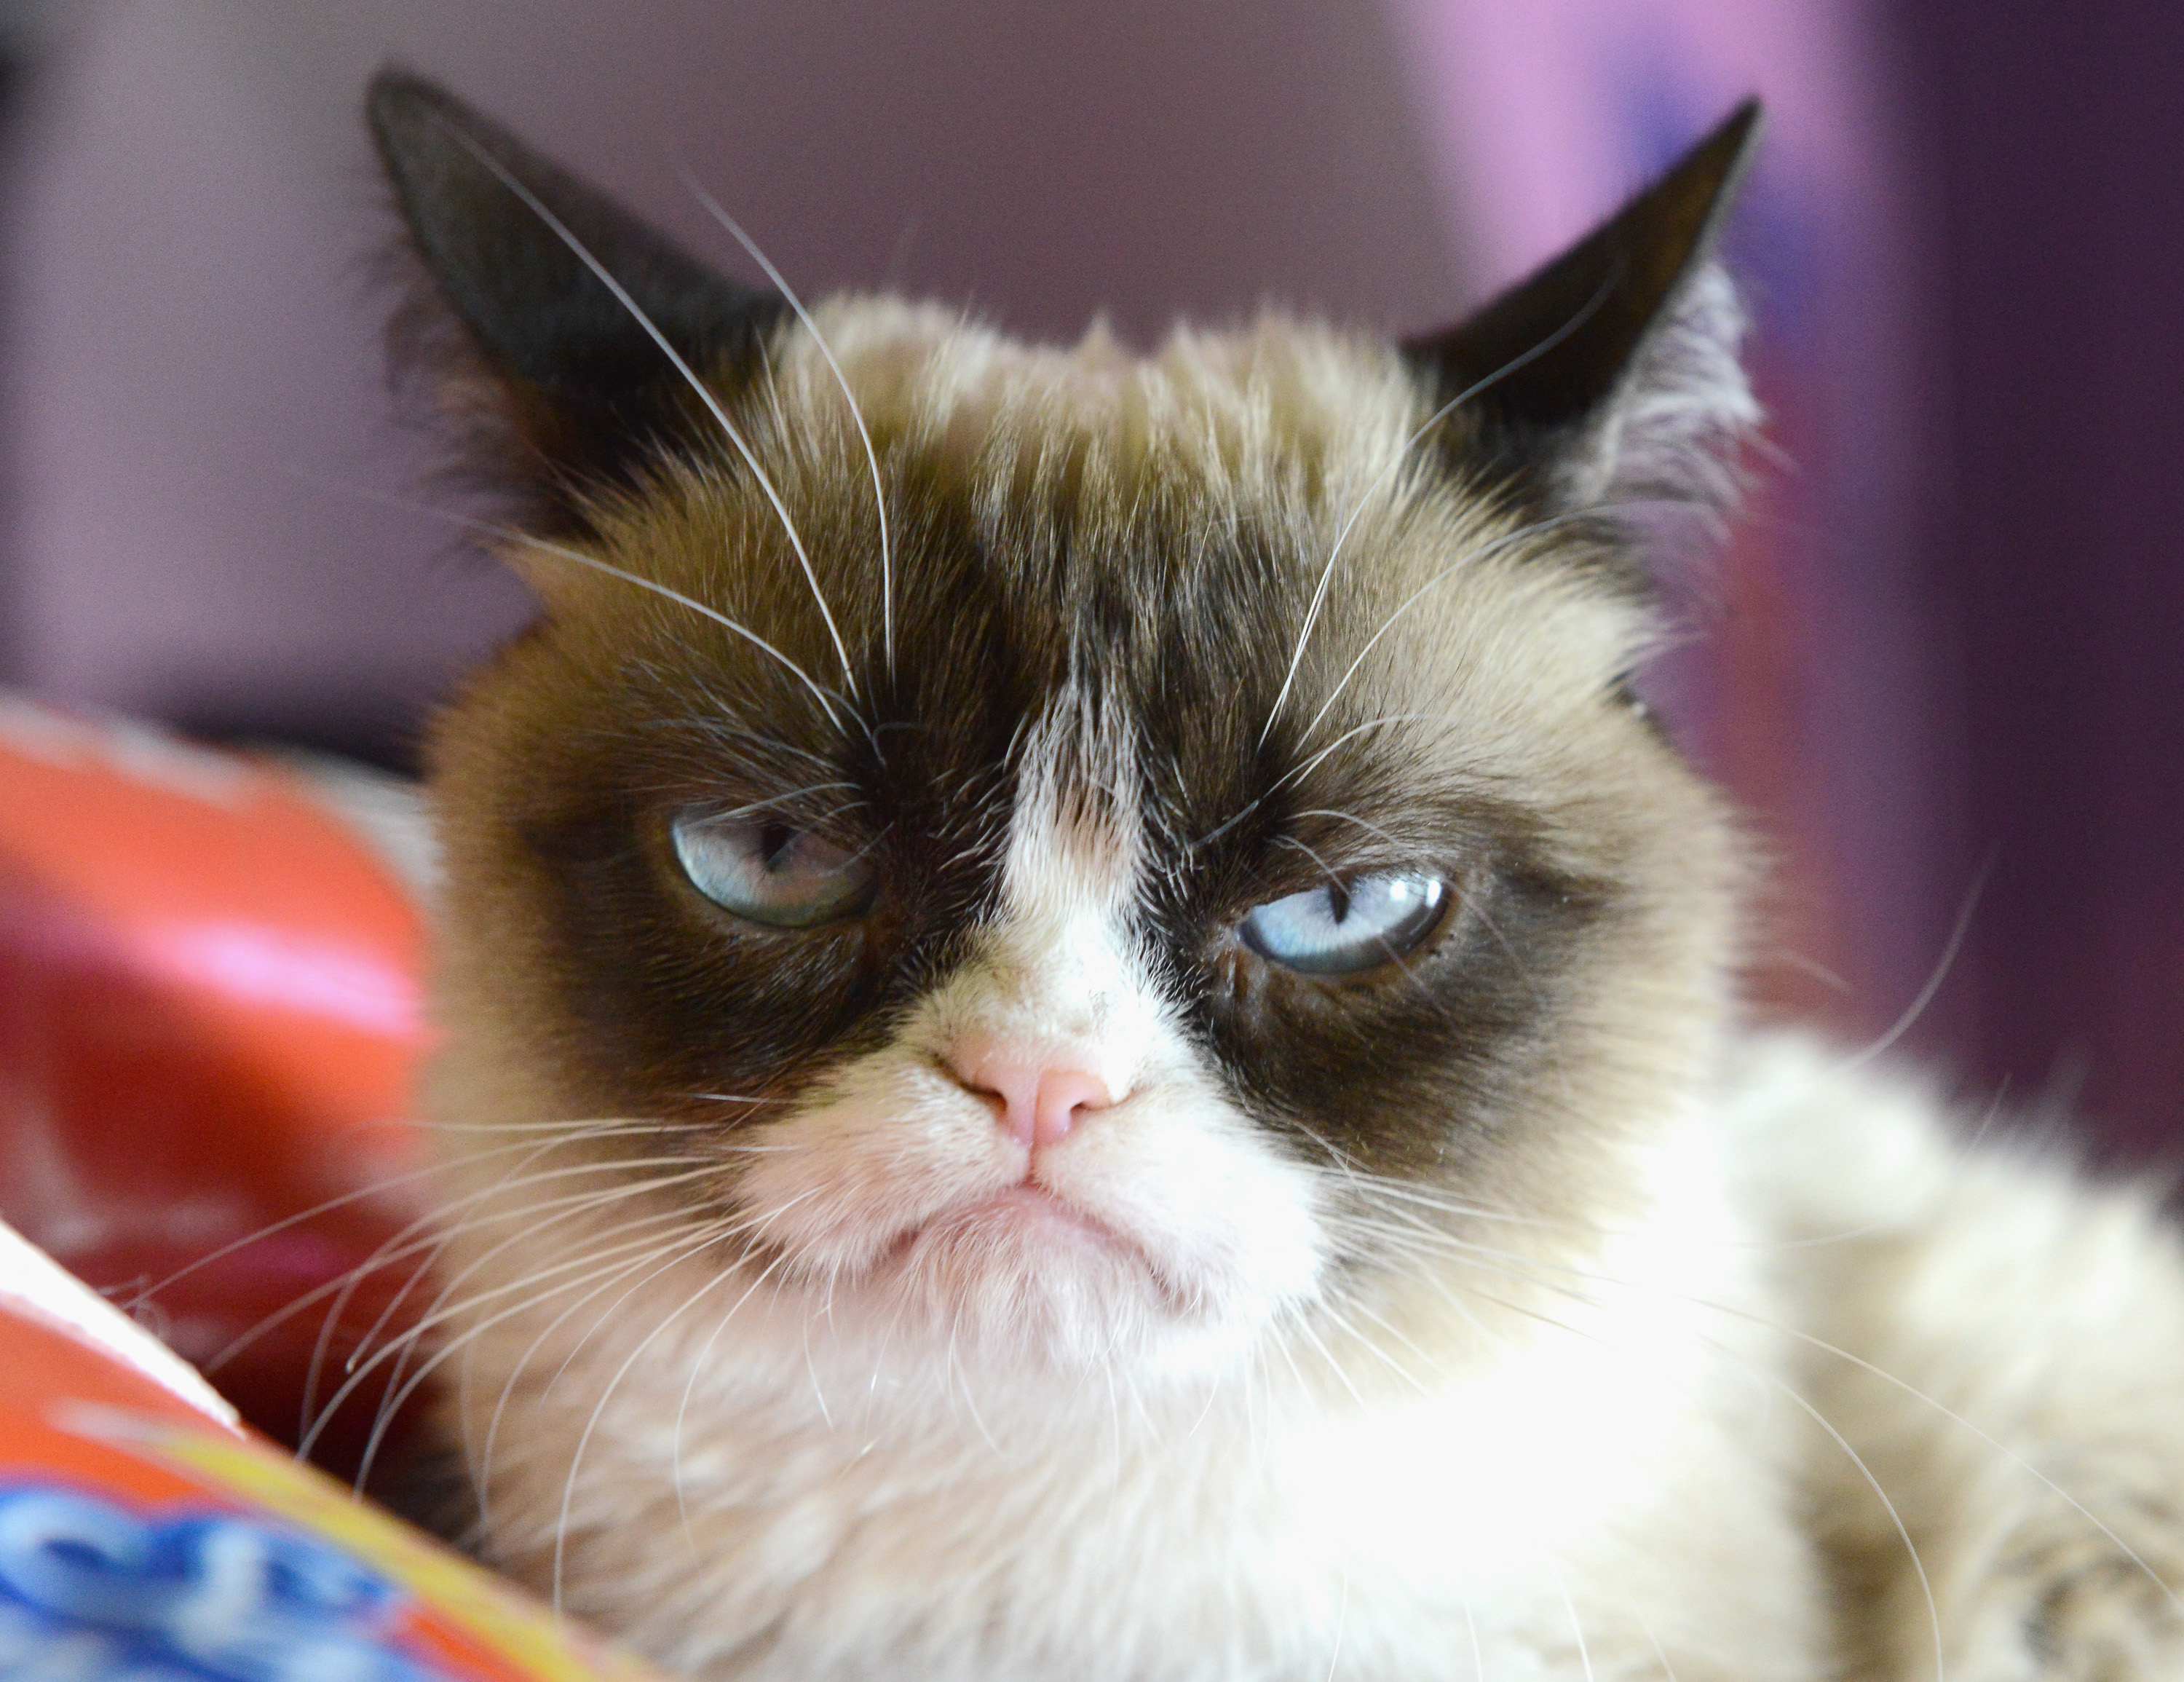
\includegraphics[width=0.75\linewidth]{image.jpg}|\\
\verb|	\caption{Dit is een voorbeeld van een figuur-float}|\\
\verb|	\label{fig:VoorbeeldFigFloat}|\\
\verb| \end{figure}|

 
 \begin{figure}[!ht]
 	\centering
 	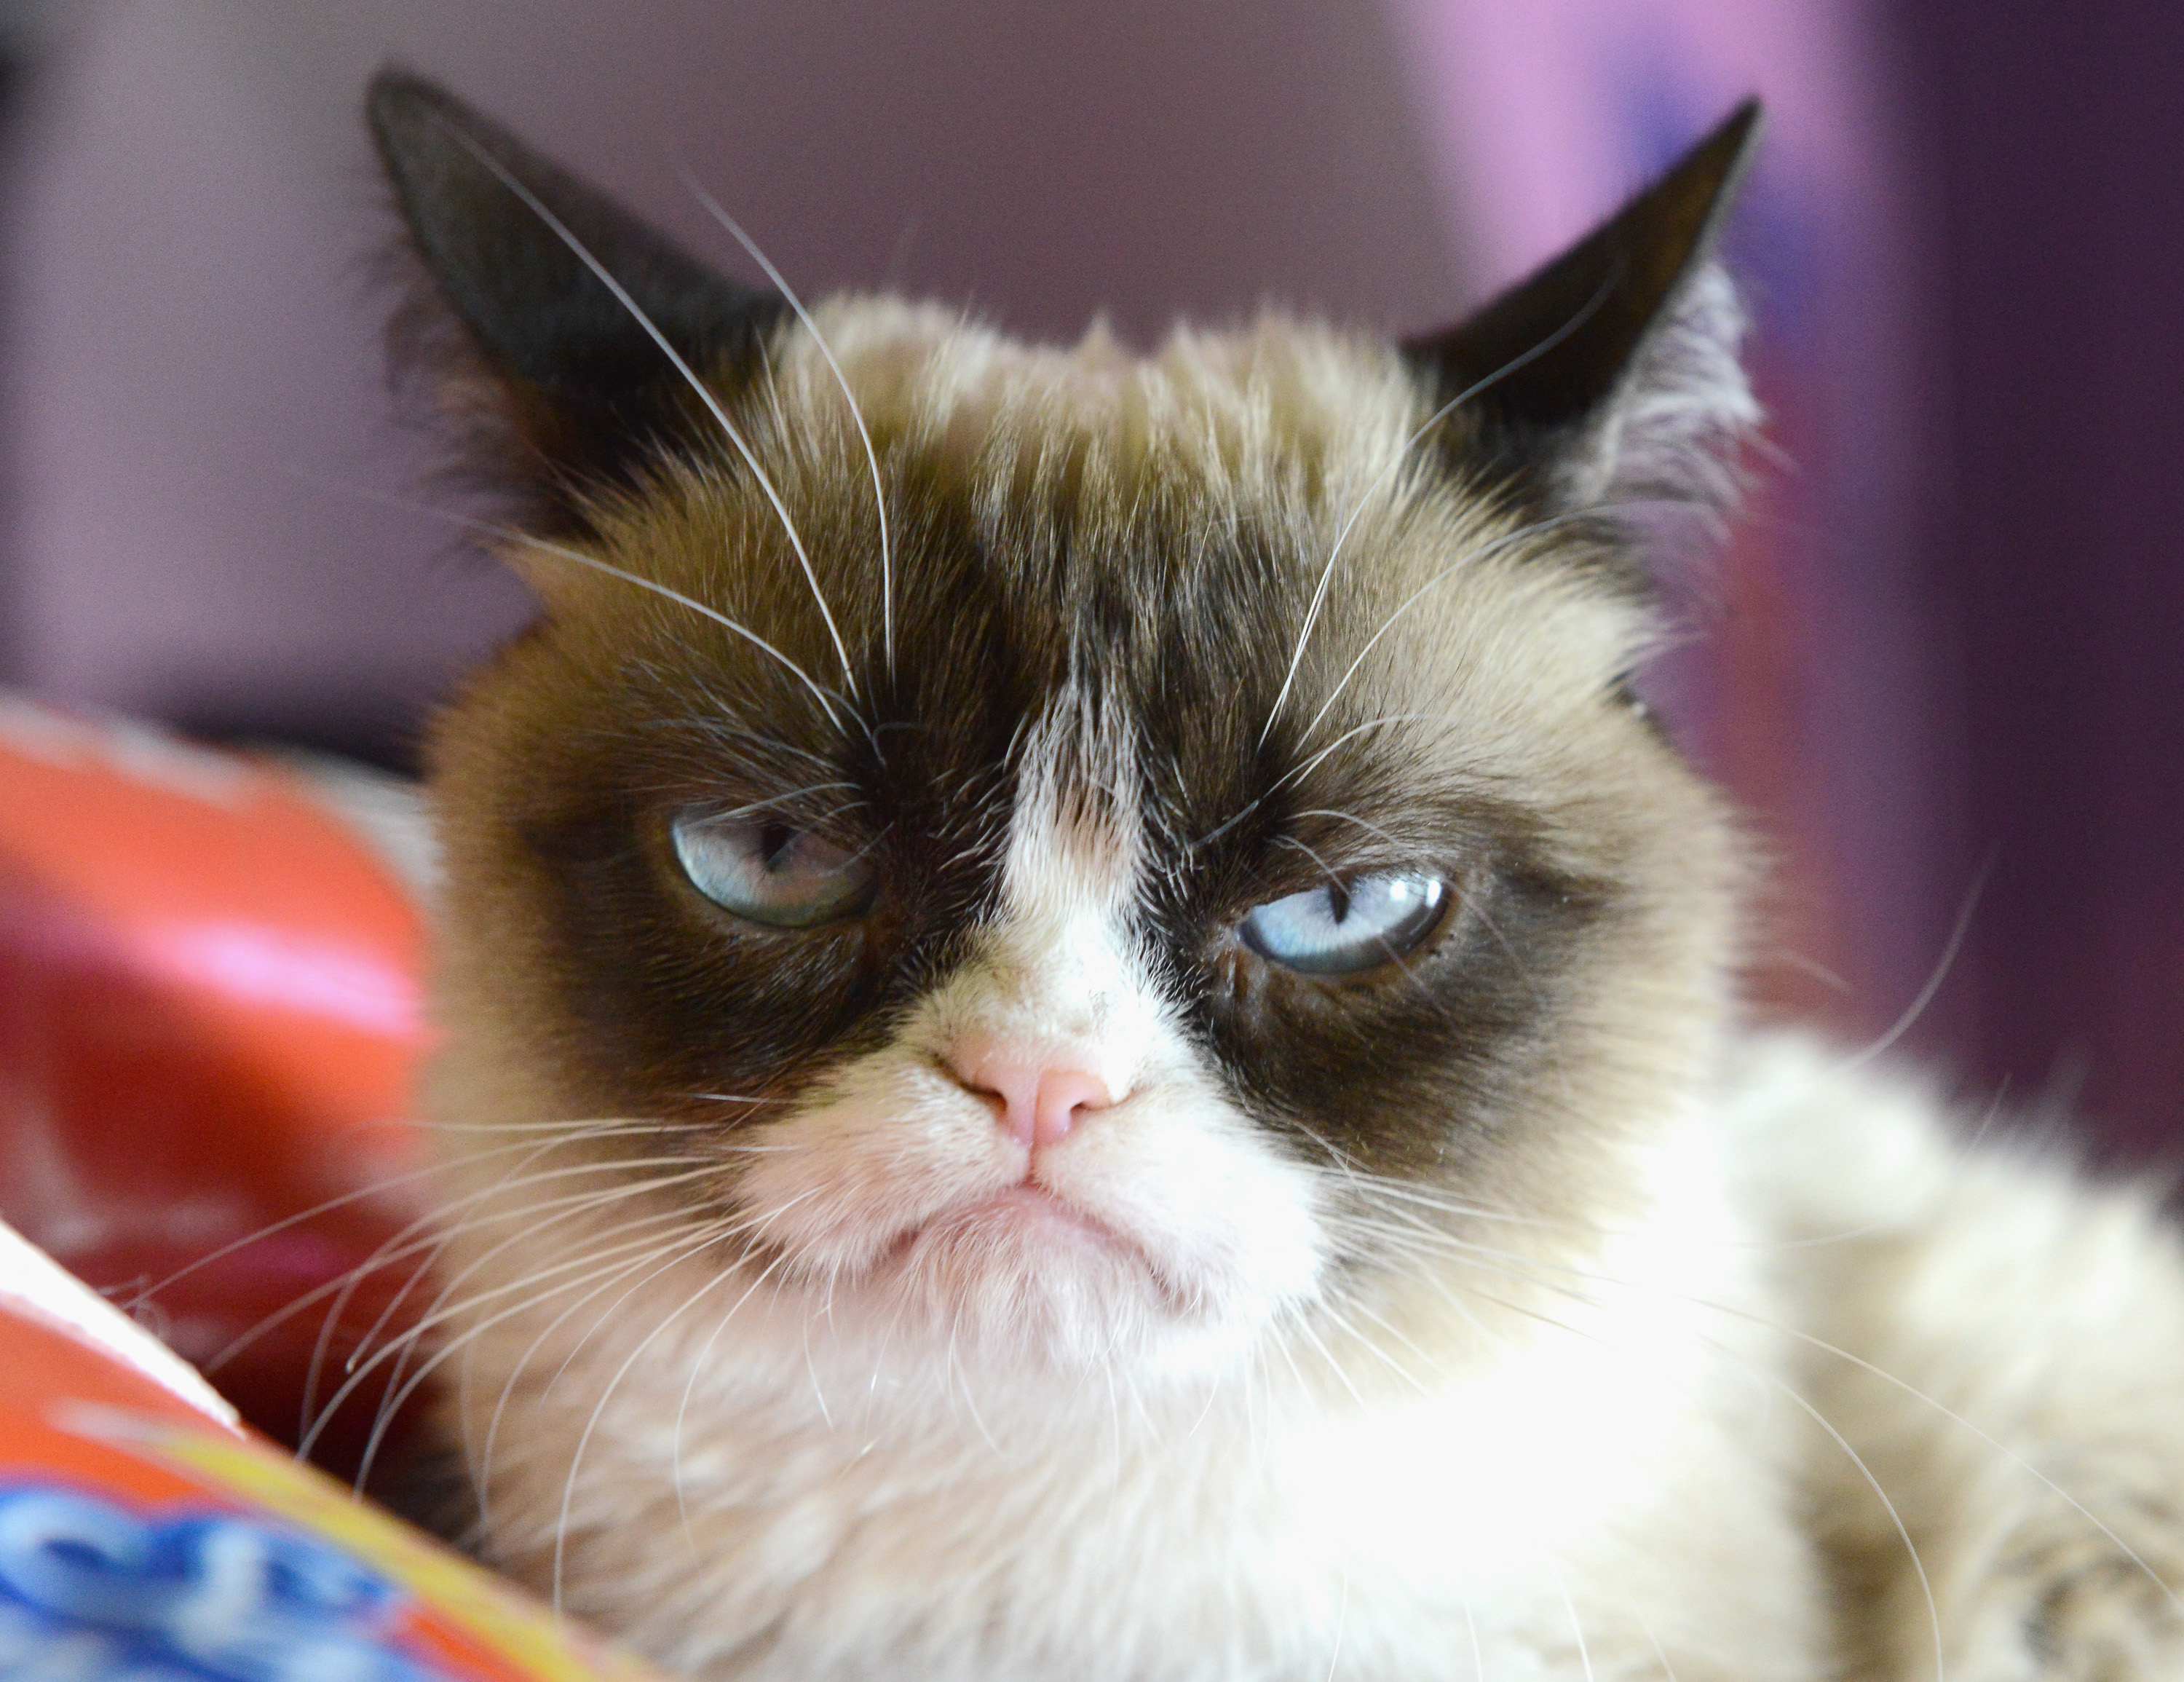
\includegraphics[width=0.75\linewidth]{image.jpg}
 	\caption{Dit is een voorbeeld van een figuur-float}
 	\label{fig:VoorbeeldFigFloat}
 \end{figure}

Tabellen worden links uitgelijnd op de bladzijde. Ook het bijschrift wordt links uitgelijnd en boven de tabel geplaatst. Na de tabelnummer volgt de beschrijving van de tabel. Tabel \ref{tab:VoorbeeldTableFloat} toont een voorbeeld van een eigen tabel. Vermijd om tabellen te kopie\"eren van andere werken, maar herwerk ze en plaats de nodige bronvermelding. De nodige syntax om tabel \ref{tab:VoorbeeldTableFloat} te generen wordt hieronder weergegeven:

\verb|\begin{table}[!ht]|\\
\verb|\caption{Dit is een voorbeeld van een tabel}|\\
\verb|\begin{tabular}{ccc}|\\
\verb|\hline|\\
\verb|Kolom 1 & Kolom 2 & Kolom 3\|\\
\verb|\hline|\\
\verb|1 & 2 & 3\\|\\
\verb|4 & 5 & 6\\|\\
\verb|\hline|\\
\verb|\end{tabular}|\\
\verb|\label{tab:VoorbeeldTableFloat}|\\
\verb|\end{table}|

Tot slot, let er op dat er expliciet naar elke tabel en figuur verwezen wordt vanuit de tekst. 

\begin{table}[!ht]
		\caption{Dit is een voorbeeld van een tabel}
	\begin{tabular}{ccc}
		\hline
		Kolom 1 & Kolom 2 & Kolom 3\\
		\hline
		1 & 2 & 3\\
		4 & 5 & 6\\
		\hline
	\end{tabular}
\label{tab:VoorbeeldTableFloat}
\end{table}
%%%%%%%%%%%%%%%%%%%%%%%%%%%%%%%%%%%%%%%%%%%%%%%%%%%%%%%%%%%%%%%%%%%% 
%                                                                 %
%                            CHAPTER                              %
%                                                                 %
%%%%%%%%%%%%%%%%%%%%%%%%%%%%%%%%%%%%%%%%%%%%%%%%%%%%%%%%%%%%%%%%%%% 
\chapter{Richtlijnen voor formules}

Er zijn twee manieren om formules in LaTeX in te voeren:

\begin{itemize}
	\item Inline: $a^2+b^2 = c^2$ (\verb|$a^2+b^2 = c^2$|)
	\item In een equation omgeving 	(\verb|\begin{equation}	a^2+b^2 = c^2	\end{equation}|):
	\begin{equation}
		a^2+b^2 = c^2
	\end{equation}

\end{itemize}

Griekse letters geef je in d.m.b. het backslash commando. Bijvoorbeeld de letter sigma $\sigma$ verkrijg je door \verb|$\sigma$| inline in te geven. Dit is analoog voor griekse letters in de equation omgeving. Een beknopte lijst van symbolen vind je op de Wikibooks pagina voor LaTeX (\href{https://nl.wikibooks.org/wiki/LaTeX/Wiskundige_formules}{link}). Alle andere nuttige informatie omtrent het gebruik van LaTeX voor formules vind je hier ook terug.
\cleardoublepage
%%%%%%%%%%%%%%%%%%%%%%%%%%%%%%%%%%%%%%%%%%%%%%%%%%%%%%%%%%%%%%%%%%%% 
%                                                                 %
%                            CHAPTER                              %
%                                                                 %
%%%%%%%%%%%%%%%%%%%%%%%%%%%%%%%%%%%%%%%%%%%%%%%%%%%%%%%%%%%%%%%%%%% 
\chapter{Richtlijnen voor referenties}

\section{Inleiding}
De referentielijst bevat de volledige lijst van literatuur en bronnen waarnaar in de tekst wordt verwezen. Door systematisch de referentielijst aan te vullen bij het schrijven van het literatuuroverzicht gaat er achteraf geen tijd verloren aan het opnieuw opzoeken van referenties.

\section{Referentiestijl}

Voor het verwijzen naar informatiebronnen wordt gebruik gemaakt van het numerisch systeem  of van het auteur-jaar systeem. Dit kies je door volgend commando in het latex bronbestand aan te passen:

\begin{itemize}
	\item numerisch (IEEE) : \verb|\bibliographystyle{ieee}|
	\item alfabetisch (APA) : \verb|\bibliographystyle{apalike}|
\end{itemize}

Plaats je bronnen in een \textit{bibtex} bestand (evt. via software zoals bv. Jabref Endnote of Mendeley), waarnaar je verwijst vanuit je thesis text a.d.h.v. het commando \verb|\cite|. Enkele links naar nuttige software in deze context:

\begin{itemize}
	\item \href{http://www.jabref.org/}{JabRef (Open Source)}
	\item \href{http://www.mendeley.com}{Mendeley (Freeware)}
	\item \href{http://www.endnote.com}{EndNote (Paid license)}
\end{itemize}

Indien je zelf een .bibtex bestand wil aanleggen dien je volgende syntax te volgen voor een tijdschriftartikel:
\clearpage
\verb|@article{hughes2005,|\\
\verb|title={Isogeometric analysis: CAD, finite elements, NURBS, exact geometry|\\ \verb|and mesh refinement},|\\
\verb|author={Hughes, Thomas JR and Cottrell, John A and Bazilevs, Yuri},|\\
\verb|journal={Computer methods in applied mechanics and engineering},|\\
\verb|volume={194},|\\
\verb|number={39},|\\
\verb|pages={4135--4195},|\\
\verb|year={2005},|\\
\verb|publisher={Elsevier}|\\
\verb|}|

Enkele voorbeelden van het gebruik van bronnen in een tekst (in APA stijl): 

Recent werd het Higgs boson experimenteel vastgesteld door Aad et al.\ \cite{aad2012} (syntax: \verb|\cite{aad2012}|). 

Als alternatief voor het discretiseren van een CAD model vooraleer een eindige elementenanalyse te kunnen toepassen, stellen Hughes et al.\ voor om de nodige elementenformulering rechtstreeks uit de NURBS beschrijving van de CAD geometrie te halen \cite{hughes2005} (syntax: \verb|\cite{hughes2005}|). Daarnaast introduceren ze tevens een k-iteratieve procedure als een verfijning van de geldende p- en h-iteratieve procedures in eindige elementen methoden \cite{cottrell2009} (syntax: \verb|\cite{cottrell2009}|).


%%%%%%%%%%%%%%%%%%%%%%%%%%%%%%%%%%%%%%%%%%%%%%%%%%%%%%%%%%%%%%%%%%% 
%                                                                 %
%                            CHAPTER                              %
%                                                                 %
%%%%%%%%%%%%%%%%%%%%%%%%%%%%%%%%%%%%%%%%%%%%%%%%%%%%%%%%%%%%%%%%%%% 

\chapter{Introduction}

blabla blabla tekst tekst.
%%%%%%%%%%%%%%%%%%%%%%%%%%%%%%%%%%%%%%%%%%%%%%%%%%%%%%%%%%%%%%%%%%% 
%                                                                 %
%                            CHAPTER                              %
%                                                                 %
%%%%%%%%%%%%%%%%%%%%%%%%%%%%%%%%%%%%%%%%%%%%%%%%%%%%%%%%%%%%%%%%%%% 

\chapter{Background information on DNA and DNA sequencing}
\label{ch:MBbackground}

\section{Biology and DNA}

\subsection{History of genetics and DNA}

\paragraph{Genetics}

\begin{wrapfigure}{R}{0.25\textwidth}
	%src: https://upload.wikimedia.org/wikipedia/commons/8/87/Gregor_Mendel_portrait.jpg
	\begin{center}
		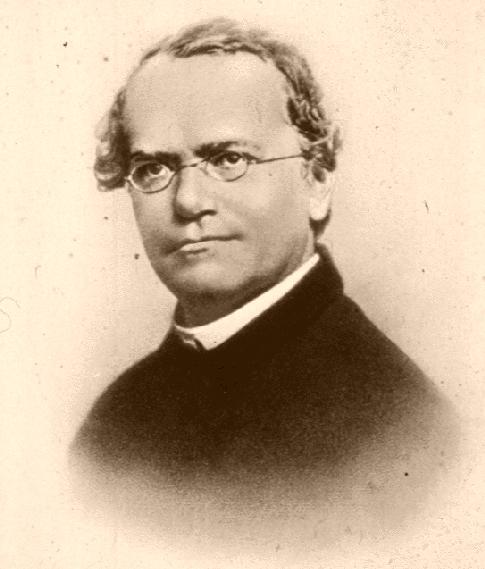
\includegraphics[width=0.20\textwidth]{background/GregorMendel.jpg}
		Gregor Mendel
	\end{center}
\end{wrapfigure}


For thousands of years, humans have observed the effects of heredity and implemented their knowledge to domesticate plants and animals. However, the science behind heredity was only started to be understood since 1859 with the publication of \emph{on the origin of species} by Charles Darwin. 

Around 1865, an Austrian monk and botanist Gregor Mendel, who studied at the university in Brno in the current Czech Republic, published his results on the hybridization studies of pea plants. He is often credited as being the father of modern genetics. In his findings, he implemented the role of \emph{factors} that influence the expression of traits. These factors later became known as \emph{genes}~\cite{Mendel}.

\paragraph{DNA}

In 1869, Swiss physician Friedrich Miescher discovered a microscopic substance in the pus of discarded surgical bandages. Later, in 1909, Phoebus Levene named this substance DeoxyriboNucleic Acid (DNA) since it is found in the nucleus of a cell and has acidic properties~\cite{Miescher}.

The full structure of DNA was discovered by Francis Crick and James Watson at the Cavendish Laboratory at the University of Cambridge~\cite{Crick}.

\subsection{Structure of DNA}

DNA, or Deoxyribonucleic Acid, is the molecule that stores the genetic information of all living organisms. It is the information that programs all of the activities in a cell.

Structurally, DNA is a polymer, which means each molecule is built up out of small repeating molecular units. In DNA, these units are called \emph{nucleotides}.

\begin{figure}[H]
	\centering
	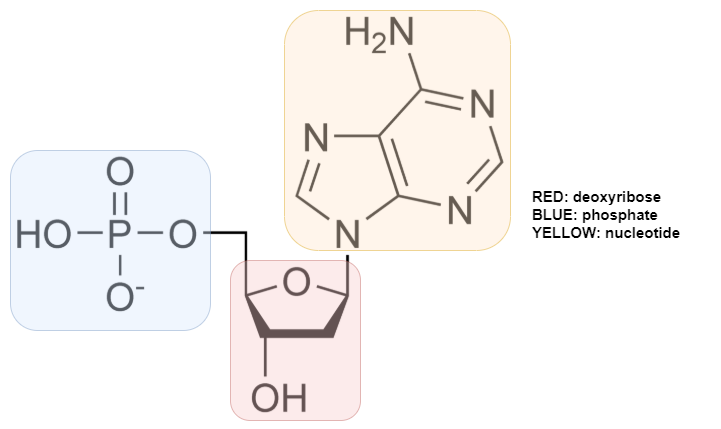
\includegraphics[width=0.75\linewidth]{background/Nucleotide.png}
	\caption{The structure of one nucleotide~\cite{Nucleotide}(modified from source).}
	\label{fig:nucleotide}
\end{figure}

Each nucleotide consists of 3 parts:

\begin{enumerate}
	\item A carbon sugar molecule called \emph{Deoxyribose}.
	\item A phosphate group to connect the Deoxyribose molecules. 
	\item One of four possible nitrogen bases: Adenine ($A$), Thymine ($T$), Cytosine ($C$) or Guanine ($G$).
\end{enumerate}

It is important to note that in most living organisms DNA does not exist as a single polymer, but rather a pair of molecules that are held tightly together. This is the famous \emph{double helix}.

\begin{figure}[H]
	%src: https://upload.wikimedia.org/wikipedia/commons/thumb/1/14/Double_stranded_DNA_with_coloured_bases.png/1024px-Double_stranded_DNA_with_coloured_bases.png
	\centering
	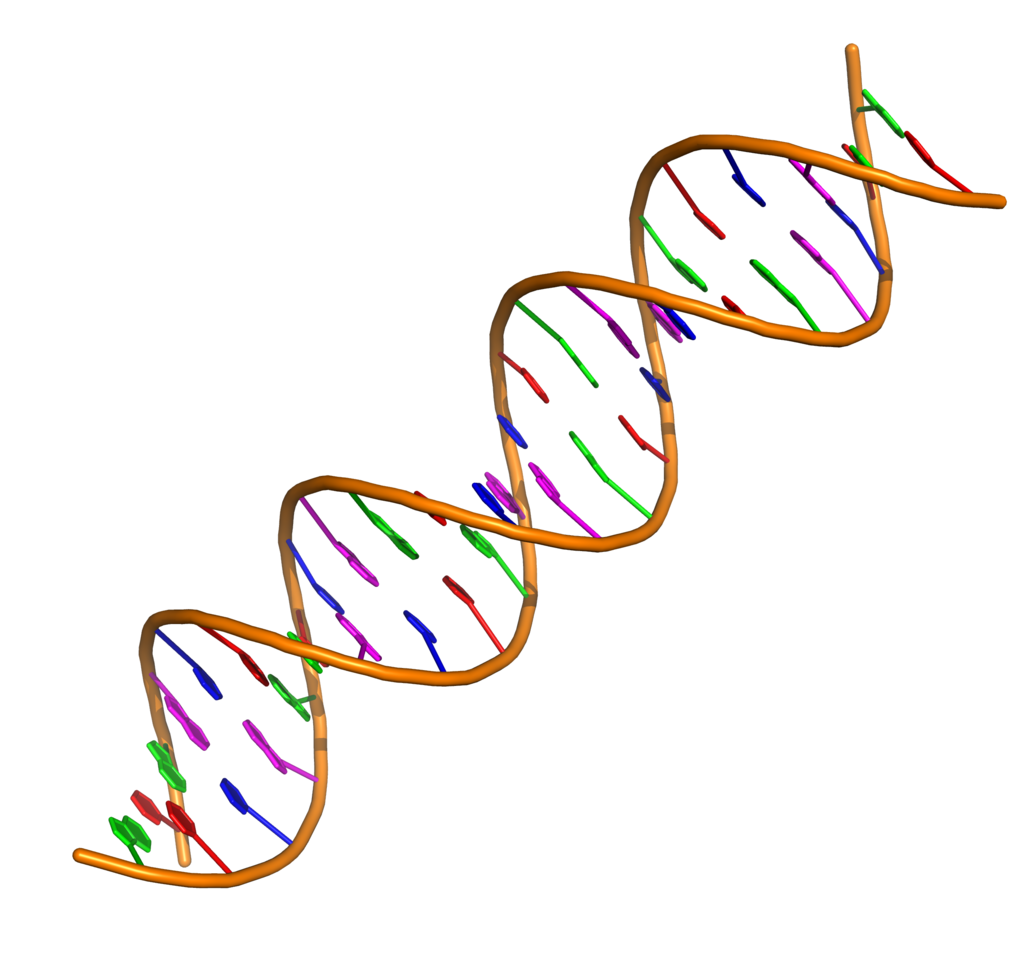
\includegraphics[width=0.3\linewidth]{background/DoubleHelix.png}
	\caption{The famous double helix~\cite{dna}.}
	\label{fig:doubleHelix}
\end{figure}

Like in any good structure, there is a need for the main support. In DNA, the sugars and phosphates bond together to form twin backbones. These sugar-phosphate bonds run down each side of the helix, but chemically in opposite directions. 

The first phosphate group, at the start of the molecule, connects to the sugar group's 5th carbon ($5'$). At the end of the structure, the 3rd carbon ($3'$) of the sugar group is unconnected. This makes a pattern typically noted as $[5' \rightarrow 3']$. Now, since the other molecule in the helix goes in the opposite direction, the pattern of the other backbone is typically noted as $[3' \rightarrow 5']$.

\begin{figure}[H]
	%src: https://upload.wikimedia.org/wikipedia/commons/thumb/e/e4/DNA_chemical_structure.svg/800px-DNA_chemical_structure.svg.png
	\centering
	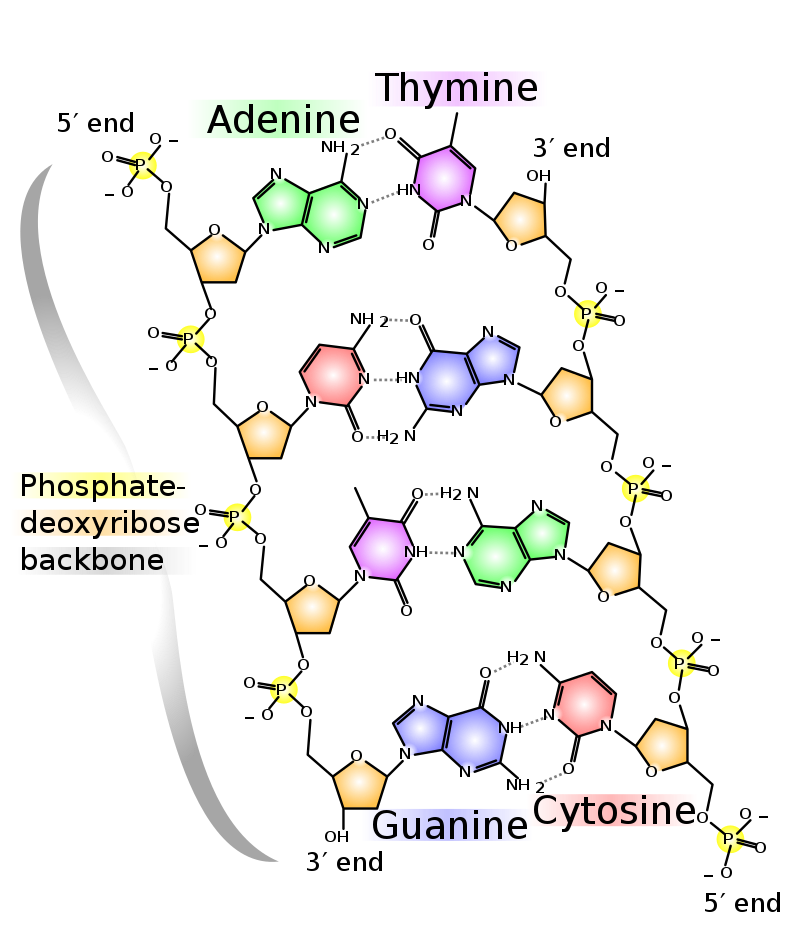
\includegraphics[width=0.5\linewidth]{background/DNAstructure.png}
	\caption{A short part of a DNA molecule containing a $[5' - ACTG - 3']$ (left) and a complementary strand of $[3' - TGAC - 5']$ (right). These 2 strands are interconnected by hydrogen bonds~\cite{dnachemical}.}
	\label{fig:DNAstructure}
\end{figure}

These two long chains are linked together by the nitrogen bases via their relatively weak hydrogen bonds, but there can't just be any pair of nitrogen bases. Adenine can only make hydrogen bonds with Thymine. Likewise, Guanine can only bond with Cytosine. These bonded nitrogen bases are called \emph{base paires}.

It is the order of these bases, which is also called the \emph{sequence}, that allows this DNA to store useful information. In this way, e.g. $AGGTCCATG$ means something completely different as a base sequence than e.g. $TTCCAGATC$.

Since each of the bases in the sequence has only one possible counterpart, you can predict what its matching counterpart will be in the opposite string. For example:

If the following sequence is known
$$[5' - AGGTCCG - 3']$$
we can deduce the sequence in the other direction as
$$[3' - TCCAGGC - 5']$$

//TODO einde zin = punt?

\subsection{DNA in the human body}

In human cells, DNA molecules can be found in the nucleus of all cells in the body. It consists of 46 very long molecules, which during cell division condense in what we call \emph{chromosomes}. The only exception is in reproductive cells (the egg cell and the sperm cell), which only have 23 chromosomes. 

The 23 chromosomes, which make up our whole DNA, are always present in pairs in the cells, making a total of 46 chromosomes. Each time, the pair consists of one chromosome from the father and the other one from the mother. 

The 23 chromosome pairs are classified in:
\begin{itemize}
	\item 22 pairs of autosomal chromosomes, marked 1 to 22 according to the length of the sequence. The longest chromosome (chromosome number-1) is 248,956,422 bases long. The shortest (chromosome number-22) is 50,818,468 bases long.
	\item In each cell, there is also an X chromosome plus an X or Y chromosome, dependent on the gender (XY for male, XX for female).
\end{itemize}


\begin{figure}[H]
	%src: https://upload.wikimedia.org/wikipedia/commons/thumb/b/b2/Karyotype.png/800px-Karyotype.png
	\centering
	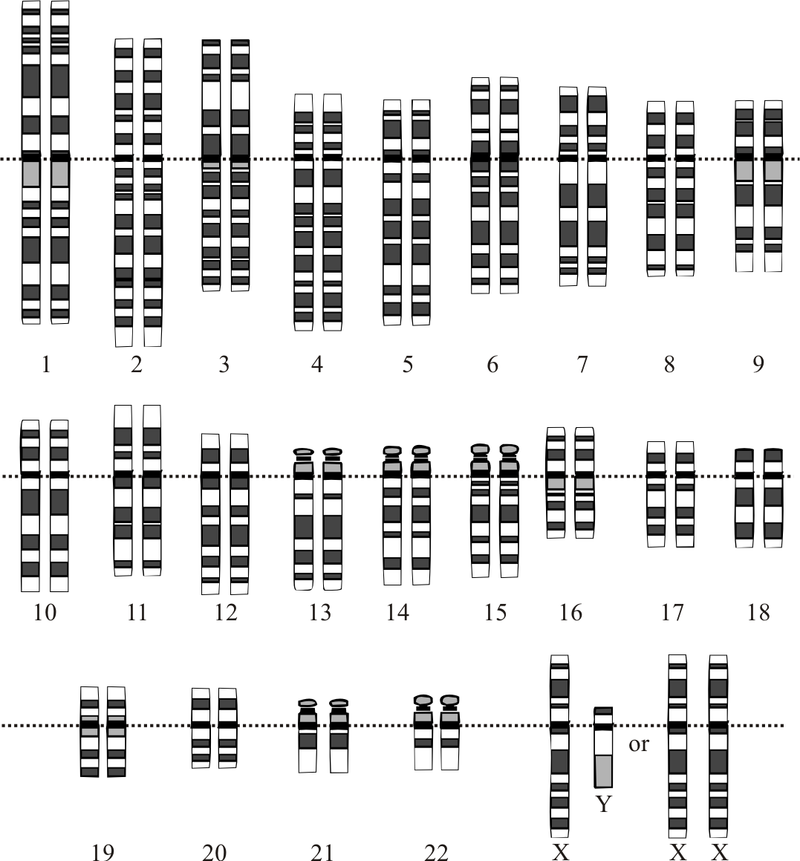
\includegraphics[width=0.5\linewidth]{background/karyotype.png}
	\caption{the 46 human chromosomes~\cite{8}.}
	\label{fig:karyotype}
\end{figure}

These chromosomes are packed tightly together in the nucleus of the cell. If all of these 46 chromosomes are put together, this makes about two times 3 billion base pairs. These 3 billion base pairs provide the assembly instructions for pretty much everything inside the cell.


\section{The Human Genome Project}

In the field of Bioinformatics, an important dataset is the \emph{Human Genome}. This is the full DNA sequence found in the Nucleus, ordered from chromosome 1 to 22, followed by the X and Y chromosome.

In October 1990, biologists in the relatively new field of molecular biology started the Human Genome Project. The goal of this project was to determine the sequence of the 3 billion base pairs that make up human DNA. This project was completed and published in 2003. So, nowadays we have a good idea of how the human genome is built up.

The Human Genome is easily found on the internet since it is publically available. One of the most often used assembly is \emph{hg19}, which was published in 2009. Since DNA has only 4 possible bases ($A$, $T$, $C$ or $G$), this can be encoded in a 2-bit representation. If this encoding is used, ideally the Human Genome is approximately 750 megabytes.

\begin{figure}[H]
	\centering
	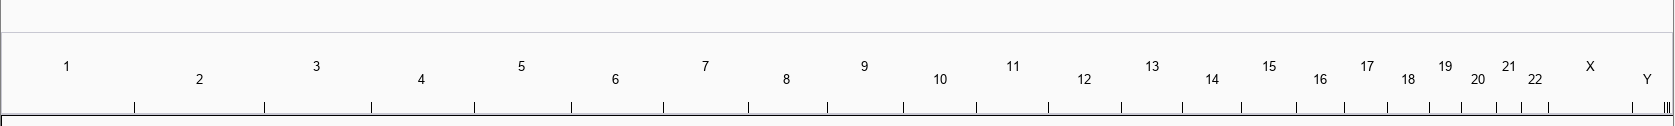
\includegraphics[width=\linewidth]{background/HG.png}
	\caption{The order and the sizes of the chromosomes of the human genome as depicted in the IGV software~\cite{IGV}.}
	\label{fig:HG}
\end{figure}

\section{Sequencing}

\subsection{The sequencing technology}

The term \emph{Sequencing} is used for all techniques to read and decipher the DNA code from a given snippet of DNA. During the last years, the techniques that sequence human DNA has changed quite a lot. For about 15 years the \emph{Next Generation Sequencing (NGS)} is the technique most often used. The biggest advantage of NGS, in comparison with other techniques, is the speed of the sequencing since it can sequence billions of short DNA molecules in parallel. In practice, this sequencing is most often done by the instruments of the company Illumina, which dominates the market (around 90\% market share).

\paragraph{How whole-genome NGS works}

\begin{enumerate}
	\item The DNA to sequence is isolated from the cells. Most often this is the whole genome.
	\item  In some cases, the isolated DNA can now be copied enzymatically. This step is repeated until there are enough copies of the same DNA. Usually, this is in the millions or billions of copies.
	
	\begin{figure}[H]
		%src: file:///D:/Erasmus/thesis/interessante%20papers/masterthesis%20BFAST%20op%20FPGA.pdf
		\centering
		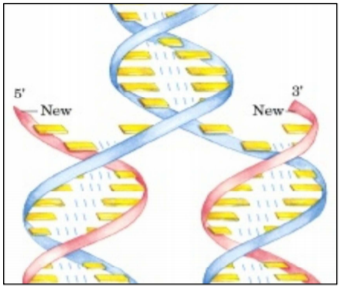
\includegraphics[width=0.3\linewidth]{background/enzymCopying.png}
		\caption{The enzymatic copying of a string of DNA. The original is unzipped, thus allowing new nucleotide bases to attach to the exposed bases~\cite{}.}
		\label{fig:enzymCopying}
	\end{figure}
	
	\item The full DNA sequence is now broken apart into small DNA molecules (100 to 1000 bases long). This is done using enzymes or high-frequency sound waves.
	\item Now the sequencing can start: a \emph{flow cell} is used where these small DNA molecules can bind to a glass surface. 
	\item Different enzymatic and chemical reactions can now be done on this flow cell through an automatic flow of reagents. The following steps are iterated until the full read has been filled in:
	\begin{enumerate}
		\item The entire flowcell is filled with nucleotides, all with different nitrogen bases. Important is that at each of these nucleotides there is a fluorescent group attached. This also makes sure no other nucleotide can bind.
		\item The fluorescent groups have a different color, dependent on the nitrogen base attached ($A$, $G$, $T$ of $C$). At this time a camera picture of the flowcell is taken and stored.
		\item After the flowcell is emptied of the loose nucleotides, another reagent flows in this flowcell. This reagent splits the fluorescent group so that in the next iteration a new nucleotide group can bind with the read.
		
		\begin{figure}[H]
			%src: file:///D:/Erasmus/thesis/interessante%20papers/masterthesis%20BFAST%20op%20FPGA.pdf
			\centering
			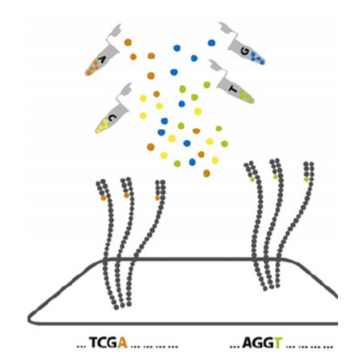
\includegraphics[width=0.5\linewidth]{background/NGS.png}
			\caption{Sequencing technology used by Illumina attaches a nucleotide with a fluorescent tag to the next base in the read, then it captures a picture to determine the base, and removes the fluorescent tag so a new nucleotide group can bind in the next iteration~\cite{}.}
			\label{fig:NGS}
		\end{figure}
	\end{enumerate}
	
	\item After the whole DNA snippets have been filled in, the machine deduces the sequence in the DNA snippet. The pictures that were taken in order during the operation show the colors released in a specific spot, and by extent the attached nitrogen base. By the means of some image processing techniques, it is quite easy to get all the sequences from all the molecules bound on the flowcell. This is called the \emph{Primary processing}.
	
	\begin{figure}[H]
		%src: PPT van Howest
		\centering
		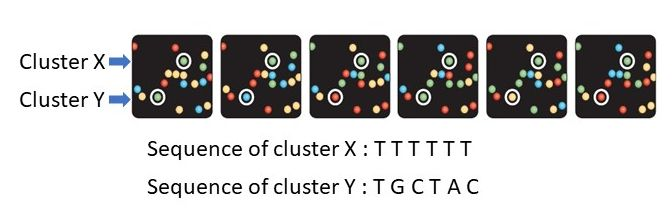
\includegraphics[width=\linewidth]{background/ImProc.jpg}
		\caption{From left to right are the pictures taken at each iteration in the flowcell. The color at that specific spot marks which nucleotide has been bound. With the use of some image processing techniques the exact sequence in that spot can be identified~\cite{pptHowest}.}
		\label{fig:ImProc}
	\end{figure}
	
	\item In the \emph{secundary processing}, the sequence is trimmed by quality, etc. The operations that are done on the read in this step are outside the scope of this thesis.
\end{enumerate}

As a result of the NGS, we get a (large) file in the FASTQ format.

\subsection{The FASTQ file format}
\label{expl:FASTQ}

Since the color of each spot observed in the camera pictures in the primary processing can have a light shift, there is a specific "uncertainty" about the correct base is in that spot. This is called the \emph{quality} of the base.

The \emph{FASTQ} file format has become the de-facto standard as output from sequencing instruments. It is a text-based format for storing both the bases in the sequence and their corresponding quality.

A FASTQ file uses four lines per sequenced DNA fragment:

\begin{enumerate}
	\item A '$@$' character followed by a sequence ID, plus an optional description. This description mostly contains the coordinate of the spot on the flowcell.
	\item \label{enumIt:fastqRaw} The sequence of DNA bases identified by the machine. This is either $A$, $G$, $C$, $T$, or $n$ when the base cannot be identified with a specific threshold certainty.
	\item A '$+$' character, optionally followed by the sequence ID (again) and an optional description.
	\item The quality values for each respective base in line~\ref{enumIt:fastqRaw}. The length of this line must be the same as the number of bases in line~\ref{enumIt:fastqRaw}.
\end{enumerate}

The quality score in memory is a value in the range $0x21$ (lowest quality) to $0x7e$ (highest quality). Since this value is represented in ASCII in the file format, this ranges from the '$!$' character to the '$\mathtt{\sim}$' character. Hereunder is a complete list of the possible values of the quality score:

\begin{lcverbatim}
!"#$%&'()*+,-./0123456789:;<=>?@ABCDEFGHIJKLMNOPQRSTUVWXYZ
[\]^_`abcdefghijklmnopqrstuvwxyz{|}~
\end{lcverbatim}


Important to note is that this quality score is logarithmic. Also, the '$@$' and '$+$' character are a possible value for the quality, so this will be something to look out for when implementing the interpreter for this file.\\

	
A FASTQ file containing a single sequence of a DNA fragment of 55 bases might look like this:


\begin{lcverbatim}
@P3018:1114
GCTACTTCCCAAGAAGCTGTTCAGAATCAGAATGAGCCGCAACTTCGGGATGAAA
+
AAAAAEEEEEEEEEEEEEEEEEEEEEEFFFFFFGGGGGIIIJJKKKKLLLLLMMM
\end{lcverbatim}

Keep in mind that a FASTQ file consists of multiple of these sequences, all stacked under each other.
	
	

%%%%%%%%%%%%%%%%%%%%%%%%%%%%%%%%%%%%%%%%%%%%%%%%%%%%%%%%%%%%%%%%%%% 
%                                                                 %
%                            CHAPTER                              %
%                                                                 %
%%%%%%%%%%%%%%%%%%%%%%%%%%%%%%%%%%%%%%%%%%%%%%%%%%%%%%%%%%%%%%%%%%% 

\chapter{Methods for DNA sequence alignment}
\label{ch:algoverzicht}


\section{DNA sequence aligning}

The human genome is used as a reference genome for all sequenced human DNA ($hg19$ is the most widely used). However, the genetic code of all humans is slightly different, which also holds true for all other organisms. Genetic sequence alignment is the science where you try to align 2 sequences with each other so that the amount of differences is minimal. In this chapter, the most frequently used algorithms are discussed.

\subsection{Alignment in general}

In genetic codes, there are 3 types of differences between the given sequence and the reference:

\begin{itemize}
	\item Insertion: one or more bases have been added in the genetic code in a specific spot.
	\item Deletion: one or more bases have been removed from the genetic code in a specific spot.
	\item Substitution: one or more bases have been substituted by other bases.
\end{itemize}

Inserts and deletions are often described by a single term, \emph{indel}.

For example: if we want to align the following sequences:
\begin{lcverbatim}
Seq1: ATATCGGC
Seq2: ATCG
\end{lcverbatim}
The alignment itself can now be done in different ways. Possible alignments are:
\begin{lcverbatim}
Alignment 1
Seq1: AtaTCgGc
Seq2: A--TC-G-
Alignment 2
Seq1: atATCGgc
Seq2: --ATCG--
\end{lcverbatim}
Which alignment that is the actual output, depends on the algorithm and the given parameters (penalty and similarity scores). The '-' character represents a base that is not present.

Keep in mind, there is no one "correct" alignment. The core of the alignment algorithms is the same each time, but the parameters of these algorithms are changed depending on the application.

\section{Local versus global alignment}
\label{S:localVSglobalAlignment}

To explain the difference between local and global alignment, we can take a look at the following example:

\begin{lcverbatim}
The 2 DNA sequences:
Seq1: TCCCAGTTTGTGTCAGGGGACACGAG
Seq2: CGCCTCGTTTTCAGCAGTTATGTGCAGATC

Alignment 1 :
Seq1: -----------tccCAGTT-TGTGTCAGgggacacgag
Seq2: cgcctcgttttcagCAGTTATGTG-CAGatc-------

Alignment 2 :
Seq1 : tcCCa-GTTTgt-GtCAGggg-acaC-GA-g
Seq2 : cgCCtcGTTTtcaG-CAGttatgtgCaGAtc
\end{lcverbatim}

Both alignments are valid but different. The first alignment is \emph{locally aligned}. This means that the similarities are prioritized in the same region, with the similarity as high as possible. On the other hand, the second alignment is \emph{globally aligned}. Here the similarities over the full length of the sequences are used for the alignment. 

In practice, the local alignment is used most often, since it can give you information of 2 sequences that do not have (approximately) the same length.

\section{Commonly used algorithms}

In this section, we will take a look at some algorithms that are used most often for DNA sequence alignment.


The most used algorithms are often categorized in 2 ways: 

\begin{itemize}
	\item local alignment versus global alignments (see Section~\ref{S:localVSglobalAlignment})
	\item dynamic algorithms versus heuristic algorithms: dynamic algorithms are exact but slow and computationally demanding, whereas heuristic algorithms are faster but are approximations and the best alignment is not guaranteed.
\end{itemize}

A schematic view of some algorithms that are used in practice can be found below:

\begin{table}[H]
	\begin{tabular}{lllll}
		\cline{1-3}
		\multicolumn{1}{|l|}{}                          & \multicolumn{1}{l|}{\textbf{Dynamic programming}} & \multicolumn{1}{l|}{\textbf{Heuristic programming}} &  &  \\ \cline{1-3}
		\multicolumn{1}{|l|}{\textbf{Local alignment}}  & \multicolumn{1}{c|}{Smith-waterman}               & \multicolumn{1}{c|}{FASTA, BLAST}                   &  &  \\ \cline{1-3}
		\multicolumn{1}{|l|}{\textbf{Global alignment}} & \multicolumn{1}{c|}{Needleman-Wunsch}             & \multicolumn{1}{c|}{X}                              &  &  \\ \cline{1-3}
		&                                                   &                                                     &  & 
	\end{tabular}
	\caption{Classification of DNA alignment algorithms}
\end{table}


Keep in mind, a lot of other claimed "algorithms" (for example BFAST, ...), are accelerated versions of the Smith-Waterman algorithm.

\subsection{Needleman-Wunsch}
Needleman and Wunch proposed a new algorithm for genetic sequence alignment in 1970, now known as the \emph{Needleman-Wunsch} (N-W) algorithm~\cite{NW}. Since this algorithm is meant for global alignment, which is rarely used in practice, further discussion of the algorithm will not be done. However, N-W has a lot of similarities with the Smith-Waterman algorithm, discussed in the next section.

\subsection{Smith-Waterman}
\label{expl:SWanalyse}
The \emph{Smith-Waterman} (S-W) algorithm was first proposed by Temple F. Smith and Michael S. Waterman in 1981\cite{SW}. It is a variation on the N-W algorithm, adapted for local alignment. It is a dynamic programming technique, so an optimal local alignment is guaranteed. \\

The core of the algorithm is a matrix fillup with data dependencies on the previous cells. An analysis of the algorithm can be found below:

\begin{enumerate}
	\item Symbols used in the analysis:
	
	Let sequences $A = a_1 a_2 a_3 \dots a_n$ and $B = b_1 b_2 b_3 \dots b_m$ be the sequences that need to be locally aligned. Here $n$ and $m$ are the lengths of the sequences $A$ and $B$
	
	\item Define the parameters: 
	
	\begin{itemize}
		\item Define $s(a,b)$ be the \emph{similarity matrix} (sometimes also called the \emph{substitution matrix}) for the two sequences. It is used for "rewarding" when $a_i = b_j$ and "punishing" when $a_i \neq b_j$.
		
		In the most general way, we define the similarity score as a matrix of values, e.g.:
		
		\begin{table}[H]
			\centering
			\begin{tabular}{|r|r|r|r|r|}
				\hline
				& \textbf{A} & \textbf{C} & \textbf{G} & \textbf{T} \\ \hline
				\textbf{A} & 3          & -3         & -3         & -3         \\ \hline
				\textbf{C} & -3         & 3          & -3         & -3         \\ \hline
				\textbf{G} & -3         & -3         & 3          & -3         \\ \hline
				\textbf{T} & -3         & -3         & -3         & 3          \\ \hline
			\end{tabular}
			
			\caption{\centering Similarity matrix example}
		\end{table}
		
		Often, there are only 2 scores used (equal or not equal). In this case, the similarity matrix can be condensed as follows:
		
		\begin{align*}
		s(a_i,b_j)=
		\begin{cases}
		+3, \quad a_i=b_j     \\
		-3, \quad a_i\neq b_j
		\end{cases}
		\end{align*}
		
		\item Define $d$ as the \emph{gap penalty} which regulates the score for an insertion or a deletion. This parameter can be:
		
		\begin{itemize}
			\item \emph{Linear}: The penalty is constant. So, in this case, it doesn't matter if the previous was also a gap or not.
			\item \emph{Affine}: An affine gap penalty considers gap opening and extension separately. For the sake of simplicity, my further implementation will not include this refinement of the algorithm. The algorithm can be extended to include this affine gap penalty, but this would make the algorithm more complex and we would limit our ability to develop possible accelerations. It is also expected to affect the DNA mapping on a reference genome. However, if we assume the size of the gaps are small, there won't be much difference in result in comparison with the linear penalty score.
		\end{itemize}
		
		
	\end{itemize}
	
	
	\item The initialization: We construct a scoring matrix $H$ with size $(n+1)\times(m+1)$. The first column and first row are initialized with $0$.
	
	For example: if we want to align the sequences A =$GGTTGACTA$ and B = $TGTTACGG$:
	
	\begin{table}[H]
		\centering
		\begin{tabular}{rrrrrrrrrr}
			&                        & T                      & G                      & T                      & T                      & A                      & C                      & G                      & G                      \\ \cline{2-10} 
			\multicolumn{1}{r|}{}  & \multicolumn{1}{r|}{0} & \multicolumn{1}{r|}{0} & \multicolumn{1}{r|}{0} & \multicolumn{1}{r|}{0} & \multicolumn{1}{r|}{0} & \multicolumn{1}{r|}{0} & \multicolumn{1}{r|}{0} & \multicolumn{1}{r|}{0} & \multicolumn{1}{r|}{0} \\ \cline{2-10} 
			\multicolumn{1}{r|}{G} & \multicolumn{1}{r|}{0} & \multicolumn{1}{r|}{}  & \multicolumn{1}{r|}{}  & \multicolumn{1}{r|}{}  & \multicolumn{1}{r|}{}  & \multicolumn{1}{r|}{}  & \multicolumn{1}{r|}{}  & \multicolumn{1}{r|}{}  & \multicolumn{1}{r|}{}  \\ \cline{2-10} 
			\multicolumn{1}{r|}{G} & \multicolumn{1}{r|}{0} & \multicolumn{1}{r|}{}  & \multicolumn{1}{r|}{}  & \multicolumn{1}{r|}{}  & \multicolumn{1}{r|}{}  & \multicolumn{1}{r|}{}  & \multicolumn{1}{r|}{}  & \multicolumn{1}{r|}{}  & \multicolumn{1}{r|}{}  \\ \cline{2-10} 
			\multicolumn{1}{r|}{T} & \multicolumn{1}{r|}{0} & \multicolumn{1}{r|}{}  & \multicolumn{1}{r|}{}  & \multicolumn{1}{r|}{}  & \multicolumn{1}{r|}{}  & \multicolumn{1}{r|}{}  & \multicolumn{1}{r|}{}  & \multicolumn{1}{r|}{}  & \multicolumn{1}{r|}{}  \\ \cline{2-10} 
			\multicolumn{1}{r|}{T} & \multicolumn{1}{r|}{0} & \multicolumn{1}{r|}{}  & \multicolumn{1}{r|}{}  & \multicolumn{1}{r|}{}  & \multicolumn{1}{r|}{}  & \multicolumn{1}{r|}{}  & \multicolumn{1}{r|}{}  & \multicolumn{1}{r|}{}  & \multicolumn{1}{r|}{}  \\ \cline{2-10} 
			\multicolumn{1}{r|}{G} & \multicolumn{1}{r|}{0} & \multicolumn{1}{r|}{}  & \multicolumn{1}{r|}{}  & \multicolumn{1}{r|}{}  & \multicolumn{1}{r|}{}  & \multicolumn{1}{r|}{}  & \multicolumn{1}{r|}{}  & \multicolumn{1}{r|}{}  & \multicolumn{1}{r|}{}  \\ \cline{2-10} 
			\multicolumn{1}{r|}{A} & \multicolumn{1}{r|}{0} & \multicolumn{1}{r|}{}  & \multicolumn{1}{r|}{}  & \multicolumn{1}{r|}{}  & \multicolumn{1}{r|}{}  & \multicolumn{1}{r|}{}  & \multicolumn{1}{r|}{}  & \multicolumn{1}{r|}{}  & \multicolumn{1}{r|}{}  \\ \cline{2-10} 
			\multicolumn{1}{r|}{C} & \multicolumn{1}{r|}{0} & \multicolumn{1}{r|}{}  & \multicolumn{1}{r|}{}  & \multicolumn{1}{r|}{}  & \multicolumn{1}{r|}{}  & \multicolumn{1}{r|}{}  & \multicolumn{1}{r|}{}  & \multicolumn{1}{r|}{}  & \multicolumn{1}{r|}{}  \\ \cline{2-10} 
			\multicolumn{1}{r|}{T} & \multicolumn{1}{r|}{0} & \multicolumn{1}{r|}{}  & \multicolumn{1}{r|}{}  & \multicolumn{1}{r|}{}  & \multicolumn{1}{r|}{}  & \multicolumn{1}{r|}{}  & \multicolumn{1}{r|}{}  & \multicolumn{1}{r|}{}  & \multicolumn{1}{r|}{}  \\ \cline{2-10} 
			\multicolumn{1}{r|}{A} & \multicolumn{1}{r|}{0} & \multicolumn{1}{r|}{}  & \multicolumn{1}{r|}{}  & \multicolumn{1}{r|}{}  & \multicolumn{1}{r|}{}  & \multicolumn{1}{r|}{}  & \multicolumn{1}{r|}{}  & \multicolumn{1}{r|}{}  & \multicolumn{1}{r|}{}  \\ \cline{2-10} 
		\end{tabular}
		\caption{\centering Example of the initialization of the scoring matrix}
	\end{table}
	
	\item Matrix fill in:
	We fill in the matrix using the following formula:
	
	\begin{align*}
	H_{ij}= max
	\begin{cases}
	H_{i-1,j-1} + s(a_i, b_j),\\
	H_{i-1,j} - d,\\
	H_{i,j-1} - d,\\
	0
	\end{cases}
	\end{align*}
	
	If we keep in mind that the value of a cell may never be lower than 0, we can represent the data dependencies in the following schematic:
	
	
	\begin{figure}[H]
		\centering
		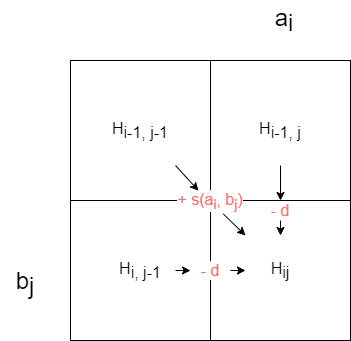
\includegraphics[width=0.5\textwidth]{ExisMethods/Dependencies_SW.png}
		\caption{Data dependencies in the $H$ matrix}
		\label{fig:DatDep}
	\end{figure}
	
	Where $s(a,b)$ and $d$ are the parameters of the algorithm. If we use the following values as an example:
	
	\begin{align*}
	s(a_i,b_j)=
	\begin{cases}
	+3, \quad a_i=b_j     \\
	-3, \quad a_i\neq b_j
	\end{cases} \qquad \text{and} \qquad d = 2
	\end{align*}
	
	We can now fill up the scoring matrix $H$:
	
	\begin{table}[H]
		\centering
		\begin{tabular}{rrrrrrrrrr}
			&                        & T                      & G                      & T                      & T                      & A                       & C                       & G                       & G                      \\ \cline{2-10} 
			\multicolumn{1}{r|}{}  & \multicolumn{1}{r|}{0} & \multicolumn{1}{r|}{0} & \multicolumn{1}{r|}{0} & \multicolumn{1}{r|}{0} & \multicolumn{1}{r|}{0} & \multicolumn{1}{r|}{0}  & \multicolumn{1}{r|}{0}  & \multicolumn{1}{r|}{0}  & \multicolumn{1}{r|}{0} \\ \cline{2-10} 
			\multicolumn{1}{r|}{G} & \multicolumn{1}{r|}{0} & \multicolumn{1}{r|}{0} & \multicolumn{1}{r|}{3} & \multicolumn{1}{r|}{1} & \multicolumn{1}{r|}{0} & \multicolumn{1}{r|}{0}  & \multicolumn{1}{r|}{0}  & \multicolumn{1}{r|}{3}  & \multicolumn{1}{r|}{3} \\ \cline{2-10} 
			\multicolumn{1}{r|}{G} & \multicolumn{1}{r|}{0} & \multicolumn{1}{r|}{0} & \multicolumn{1}{r|}{3} & \multicolumn{1}{r|}{1} & \multicolumn{1}{r|}{0} & \multicolumn{1}{r|}{0}  & \multicolumn{1}{r|}{0}  & \multicolumn{1}{r|}{3}  & \multicolumn{1}{r|}{6} \\ \cline{2-10} 
			\multicolumn{1}{r|}{T} & \multicolumn{1}{r|}{0} & \multicolumn{1}{r|}{3} & \multicolumn{1}{r|}{1} & \multicolumn{1}{r|}{6} & \multicolumn{1}{r|}{4} & \multicolumn{1}{r|}{2}  & \multicolumn{1}{r|}{0}  & \multicolumn{1}{r|}{1}  & \multicolumn{1}{r|}{4} \\ \cline{2-10} 
			\multicolumn{1}{r|}{T} & \multicolumn{1}{r|}{0} & \multicolumn{1}{r|}{3} & \multicolumn{1}{r|}{1} & \multicolumn{1}{r|}{4} & \multicolumn{1}{r|}{9} & \multicolumn{1}{r|}{7}  & \multicolumn{1}{r|}{5}  & \multicolumn{1}{r|}{3}  & \multicolumn{1}{r|}{2} \\ \cline{2-10} 
			\multicolumn{1}{r|}{G} & \multicolumn{1}{r|}{0} & \multicolumn{1}{r|}{1} & \multicolumn{1}{r|}{6} & \multicolumn{1}{r|}{4} & \multicolumn{1}{r|}{7} & \multicolumn{1}{r|}{6}  & \multicolumn{1}{r|}{4}  & \multicolumn{1}{r|}{8}  & \multicolumn{1}{r|}{6} \\ \cline{2-10} 
			\multicolumn{1}{r|}{A} & \multicolumn{1}{r|}{0} & \multicolumn{1}{r|}{0} & \multicolumn{1}{r|}{4} & \multicolumn{1}{r|}{3} & \multicolumn{1}{r|}{5} & \multicolumn{1}{r|}{10} & \multicolumn{1}{r|}{8}  & \multicolumn{1}{r|}{6}  & \multicolumn{1}{r|}{5} \\ \cline{2-10} 
			\multicolumn{1}{r|}{C} & \multicolumn{1}{r|}{0} & \multicolumn{1}{r|}{0} & \multicolumn{1}{r|}{2} & \multicolumn{1}{r|}{1} & \multicolumn{1}{r|}{3} & \multicolumn{1}{r|}{8}  & \multicolumn{1}{r|}{13} & \multicolumn{1}{r|}{11} & \multicolumn{1}{r|}{9} \\ \cline{2-10} 
			\multicolumn{1}{r|}{T} & \multicolumn{1}{r|}{0} & \multicolumn{1}{r|}{3} & \multicolumn{1}{r|}{1} & \multicolumn{1}{r|}{5} & \multicolumn{1}{r|}{4} & \multicolumn{1}{r|}{6}  & \multicolumn{1}{r|}{11} & \multicolumn{1}{r|}{10} & \multicolumn{1}{r|}{8} \\ \cline{2-10} 
			\multicolumn{1}{r|}{A} & \multicolumn{1}{r|}{0} & \multicolumn{1}{r|}{1} & \multicolumn{1}{r|}{0} & \multicolumn{1}{r|}{3} & \multicolumn{1}{r|}{2} & \multicolumn{1}{r|}{7}  & \multicolumn{1}{r|}{9}  & \multicolumn{1}{r|}{8}  & \multicolumn{1}{r|}{7} \\ \cline{2-10} 
		\end{tabular}
		\caption{\centering Example of a populated scoring matrix}
	\end{table}
	
	
	\item Traceback: We start at the cell with the highest score in the matrix $H$. Starting here we only move left, up or diagonally (left-up) to the cell on which the value in the cell was based until we hit a cell with value $0$.
	
	
	\begin{table}[H]
		\centering
		\begin{tabular}{rrrrrrrrrr}
			&                        & T                                              & G                                              & T                                              & T                                              & A                                               & C                                               & G                       & G                      \\ \cline{2-10} 
			\multicolumn{1}{r|}{}  & \multicolumn{1}{r|}{0} & \multicolumn{1}{r|}{0}                         & \multicolumn{1}{r|}{0}                         & \multicolumn{1}{r|}{0}                         & \multicolumn{1}{r|}{0}                         & \multicolumn{1}{r|}{0}                          & \multicolumn{1}{r|}{0}                          & \multicolumn{1}{r|}{0}  & \multicolumn{1}{r|}{0} \\ \cline{2-10} 
			\multicolumn{1}{r|}{G} & \multicolumn{1}{r|}{0} & \multicolumn{1}{r|}{\cellcolor[HTML]{FFCCC9}0} & \multicolumn{1}{r|}{3}                         & \multicolumn{1}{r|}{1}                         & \multicolumn{1}{r|}{0}                         & \multicolumn{1}{r|}{0}                          & \multicolumn{1}{r|}{0}                          & \multicolumn{1}{r|}{3}  & \multicolumn{1}{r|}{3} \\ \cline{2-10} 
			\multicolumn{1}{r|}{G} & \multicolumn{1}{r|}{0} & \multicolumn{1}{r|}{0}                         & \multicolumn{1}{r|}{\cellcolor[HTML]{DAE8FC}3} & \multicolumn{1}{r|}{1}                         & \multicolumn{1}{r|}{0}                         & \multicolumn{1}{r|}{0}                          & \multicolumn{1}{r|}{0}                          & \multicolumn{1}{r|}{3}  & \multicolumn{1}{r|}{6} \\ \cline{2-10} 
			\multicolumn{1}{r|}{T} & \multicolumn{1}{r|}{0} & \multicolumn{1}{r|}{3}                         & \multicolumn{1}{r|}{1}                         & \multicolumn{1}{r|}{\cellcolor[HTML]{DAE8FC}6} & \multicolumn{1}{r|}{4}                         & \multicolumn{1}{r|}{2}                          & \multicolumn{1}{r|}{0}                          & \multicolumn{1}{r|}{1}  & \multicolumn{1}{r|}{4} \\ \cline{2-10} 
			\multicolumn{1}{r|}{T} & \multicolumn{1}{r|}{0} & \multicolumn{1}{r|}{3}                         & \multicolumn{1}{r|}{1}                         & \multicolumn{1}{r|}{4}                         & \multicolumn{1}{r|}{\cellcolor[HTML]{DAE8FC}9} & \multicolumn{1}{r|}{7}                          & \multicolumn{1}{r|}{5}                          & \multicolumn{1}{r|}{3}  & \multicolumn{1}{r|}{2} \\ \cline{2-10} 
			\multicolumn{1}{r|}{G} & \multicolumn{1}{r|}{0} & \multicolumn{1}{r|}{1}                         & \multicolumn{1}{r|}{6}                         & \multicolumn{1}{r|}{4}                         & \multicolumn{1}{r|}{\cellcolor[HTML]{DAE8FC}7} & \multicolumn{1}{r|}{6}                          & \multicolumn{1}{r|}{4}                          & \multicolumn{1}{r|}{8}  & \multicolumn{1}{r|}{6} \\ \cline{2-10} 
			\multicolumn{1}{r|}{A} & \multicolumn{1}{r|}{0} & \multicolumn{1}{r|}{0}                         & \multicolumn{1}{r|}{4}                         & \multicolumn{1}{r|}{3}                         & \multicolumn{1}{r|}{5}                         & \multicolumn{1}{r|}{\cellcolor[HTML]{DAE8FC}10} & \multicolumn{1}{r|}{8}                          & \multicolumn{1}{r|}{6}  & \multicolumn{1}{r|}{5} \\ \cline{2-10} 
			\multicolumn{1}{r|}{C} & \multicolumn{1}{r|}{0} & \multicolumn{1}{r|}{0}                         & \multicolumn{1}{r|}{2}                         & \multicolumn{1}{r|}{1}                         & \multicolumn{1}{r|}{3}                         & \multicolumn{1}{r|}{8}                          & \multicolumn{1}{r|}{\cellcolor[HTML]{34CDF9}13} & \multicolumn{1}{r|}{11} & \multicolumn{1}{r|}{9} \\ \cline{2-10} 
			\multicolumn{1}{r|}{T} & \multicolumn{1}{r|}{0} & \multicolumn{1}{r|}{3}                         & \multicolumn{1}{r|}{1}                         & \multicolumn{1}{r|}{5}                         & \multicolumn{1}{r|}{4}                         & \multicolumn{1}{r|}{6}                          & \multicolumn{1}{r|}{11}                         & \multicolumn{1}{r|}{10} & \multicolumn{1}{r|}{8} \\ \cline{2-10} 
			\multicolumn{1}{r|}{A} & \multicolumn{1}{r|}{0} & \multicolumn{1}{r|}{1}                         & \multicolumn{1}{r|}{0}                         & \multicolumn{1}{r|}{3}                         & \multicolumn{1}{r|}{2}                         & \multicolumn{1}{r|}{7}                          & \multicolumn{1}{r|}{9}                          & \multicolumn{1}{r|}{8}  & \multicolumn{1}{r|}{7} \\ \cline{2-10} 
		\end{tabular}
		\caption{\centering A traceback in S-W. For example, the 13 in the blue colored cell is based on the cell with value 10 in on the left-up diagonal (match). Therefore, the path will jump to the cell with value 10. This is repeated until a 0 cell is hit.}
	\end{table}
	
	From this traceback we can now deduce the following alignment:
	
\begin{lcverbatim}
GTT-AC
||||||
GTTGAC
\end{lcverbatim}
	
	This alignment is the output of our algorithm.
	
\end{enumerate}

\section{Problem definition}

\subsection{Mapping to a reference genome}

From the DNA sequencing machines, we get a big amount of reads in the FASTQ format. We should note that all these reads are worthless without a proper interpretation.

In most cases, the first step in the analysis of the reads is knowing from which part of the genome it's derived. Typically, the read is compared with the whole genome in a local alignment, for example using the Smith-Waterman algorithm. As an output, we would get the position in the human genome and an alignment with its score (how well the sequence fits in that spot). This practice is commonly referred to as \emph{Mapping to reference genome}.

Since the reads from DNA sequencing machines are 75 to 300 bases long, and the whole human genome is approximately 3 billion bases, this comparison is computationally a very intensive task. If we analyze the S-W algorithm (as we have done in Subsection~\ref{expl:SWanalyse}), we can see that the value of each cell in the matrix is only dependent on the left-upmost 3 cells. Therefore, it leads us to believe that this algorithm can be accelerated on other hardware solutions such as an FPGA (which will be discussed in Chapter~\ref{ch:Platforms}) since S-W is heavily parallelizable.

In most clinical applications where mapping to a human reference genome is used, the number of reads to be compared with the genome is in the millions.

\begin{figure}[H]
	\centering
	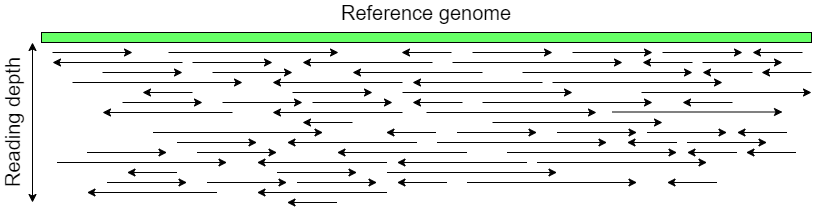
\includegraphics[width=0.95\textwidth]{problemDefinition/MappingRefGen.png}
	\caption{Mapping to a reference genome. The direction of the read is represented by arrows}
	\label{fig:mapRefGen}
\end{figure}

Since the read can be from the complementary DNA molecule in the double helix, the sequences can be in forward $[5' \rightarrow 3']$ direction, or in complementary $[3' \rightarrow 5']$ direction. To transform that read to the used reference genome direction we need to perform the following changes to the read to make its reverse complementary:
\begin{enumerate}
	\item The bases should be changed to their corresponding base in the base pair;
	\item The sequence should be reversed.
\end{enumerate}
We have no way of knowing in which direction the read is taken, both the forward and the backward possibility should be compared with the reference and the best-aligned version of these two should be chosen.

Please note, in most normal cases we can assume the distribution of reads is practically uniform. Therefore, each base in the human genome will be covered by a statistically expected amount of reads. This amount is referred to as the \emph{reading depth}.


\subsection{The SAM and BAM file format}
\label{expl:SAM}

As a convention, the output of mapping algorithms is in a \emph{SAM} (Sequence Alignment Map) or \emph{BAM} (Binary Alignment Map) file format. The BAM file format is just a compressed version of the SAM format, but the SAM format is more readable, which makes it easier for troubleshooting. There are many tools to transform a SAM to BAM file already, so in this thesis, we will focus on the SAM format. A SAM file consists of two sections: a header and an alignment section~\cite{SAM}.

%src:http://samtools.github.io/hts-specs/SAMv1.pdf

\subsubsection{Header}
The header is used for information that is independent of the alignments, such as the name of the used algorithm, reference genome, used commands during generation, etc.
The header must be at the beginning of the file, before the alignment section. Each line of the header field must start with an '@' character, so these lines are easily distinguished from lines in the alignment section.

\subsubsection{Alignment Section}
Each line in the alignment section represents one mapped sequence and consists of 11 mandatory and some optional fields, which are separated with a tab.

The 11 mandatory fields are:
\begin{enumerate}
	
	\item \textbf{Qname}: this is the name of the query (the sequence to match) and can be found on the first line of the FASTQ file, which is the input to the mapping algorithm.
	
	\item \textbf{FLAG}: a combination of bitwise flags where each bit has a specific interpretation. It consists of 11 bits, but for basic alignments only 2 fields are important:
	\begin{itemize}
		\item bit 2 (binary: $00000000X00$, integer value 4) is set to $1$ if the sequence is unmapped or the map is not found
		\item bit 4 (binary: $000000X0000$, integer value 16) is set to $1$ if the sequence has been mapped as its reverse complement.
	\end{itemize}
	
	\item \textbf{Rname}: the name of the reference genome. This can be found on the first line of the FASTA file, where the reference genome is stored. If the read is unmapped, this field contains a '*' character
	
	\item \textbf{Pos}: the position of the leftmost base in the alignment. Keep in mind that the indexing of the reference starts with 1 for the first base.
	
	\item \textbf{MapQ}: the mapping quality, which indicates how good the sequence fits in the specific position. This can be any value between 0 and 254. Value 255 is a reserved value to represent an unavailable quality.
	
	\item \textbf{CIGAR}, which stands for \textit{Concise Idiosyncratic Gapped Alignment Report}. It is a string that indicates where the matches (M), insertions (I), and deletions (D) occur. For example, if the CIGAR states $3M1I6M2D10M$ this means from left to right: 3 matches, then an insertion, followed by 6 matches, 2 deletions, and finally 10 matches. In case the sequence is unmapped, this field should be filled with a '*' character
	
	\item \textbf{Rnext}: reference sequence name of the primary alignment of the text read in the template. For this thesis, we will fill this field with a '*' character. 
	
	\item \textbf{Pnext}: the position of the primary alignment of the next read in the template. For this thesis, we will fill this field with a '0' character.
	
	\item \textbf{Tlen}: the observed template length, from the first till last mapped base. For this thesis, we will fill this field with a '0' character.
	
	\item \textbf{Seq}: the full sequence. This can be found in the FASTQ file on the second line.
	
	\item \textbf{Qual}: the qualities of the sequence, also given by the FASTQ file on the fourth line.
	
\end{enumerate}

An example of one line in a SAM file:
\begin{lcverbatim}
SRR11   0   MN98   25   254   7M   *   0   0   GTTAAAG   BBBBBCB
\end{lcverbatim}
In this example:
\begin{itemize}
	\item \textbf{Qname}: the name of the sequence: $SRR11$.
	\item \textbf{FLAG}: this read is matched in the $[5' -> 3']$ direction.
	\item \textbf{Rname}: the name of the reference genome is $MN98$.
	\item \textbf{Pos}: the match is found at the 25th base of the reference genome.
	\item \textbf{MapQ}: the mapping quality is 254.
	\item \textbf{CIGAR}: $7M$, so a perfect match.
	\item \textbf{Rnext, Pnext and Tlen}: data not provided.
	\item \textbf{Seq and Qual}: the sequence is $GTTAAAG$ with quality $BBBBBCB$.
\end{itemize}

\subsection{Clinical application}

In virtually all sequencing applications DNA alignment and reference mapping is needed. Applications which involve whole genome sequencing in particular are hampered by a long computational analysis time.

We will discuss two clinical applications as examples to genome mapping.

\begin{enumerate}
	\item \textbf{\emph{NIPT} (non-invasive prenatal testing), a test for detecting genetic defects in a foetus.}\newline
	During or after conception, DNA can be lost or gained in the fertilized egg cell. This can result in a severe syndrome of the child. For example, Down syndrome is caused by a trisomy of chromosome 21. Normally all chromosomes are present twice in each cell, one from the mother and the other from the father. In Down syndrome patients something went wrong during cell division at the very early stage of development, and the fetus has in its cells three times chromosome 21. 
	Because chromosome 21 is quite small and does not contain that many genes, the child can survive, though with typical mental and clinical problems~\cite{Down}.
	
	\begin{figure}[H]
			\centering
		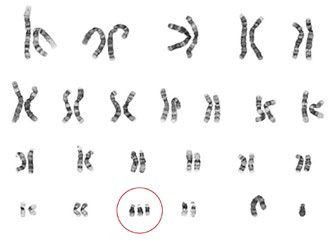
\includegraphics[width=0.45\textwidth]{clinicalAppl/trisomy21.jpg}
		\caption{Chromosomes of a patient with trisomy 21 (Down Syndrome). The trisomy of chromosome-21 is encircled~\cite{niptArtikel}.}
		\label{fig:tri21}
	\end{figure}
	
	
	Before high throughput DNA sequencing technologies were available like they are today, testing if a fetus has a trisomy-21 could only be done by taking a small amount of amniotic fluid (fluid around the fetus). However, to obtain this fluid there was a need for a risky invasive procedure (called \emph{amniocentesis}) leading sometimes to the termination of the pregnancy.
	
	It is known that small amounts of DNA of the fetus are present in the blood of the mother, in the cell-free DNA (\emph{cfDNA}) which we find in the blood plasma (the clear, aqueous part of the blood). The blood plasma is used by our body to transport 'waste', including DNA from cells that were broken down. When fetal cells die, which is a normal process, the building blocks of these cells are transported in the plasma of the blood from the mother, included small DNA fragments from the fetus~\cite{NIPT}.
	
	\emph{NIPT} (non-invasive prenatal testing) is used to analyze DNA derived from the mother's blood. A large number of short cfDNA fragments are sequenced at random.  Then, each sequence is mapped to the whole human genome to find out where it comes from. Finally, the distribution of these reads is calculated. If we observe a higher frequency of reads as compared to normal individuals coming from chromosome-21, it is almost certain that the fetus has Down's syndrome~\cite{NIPT}.
	
	\begin{figure}[H]
		%src: https://mail.google.com/mail/u/0/#search/nipt/FMfcgxwHMsQcgsbNLGvDkDqXLjxnNdWR?projector=1&messagePartId=0.1
		\centering
		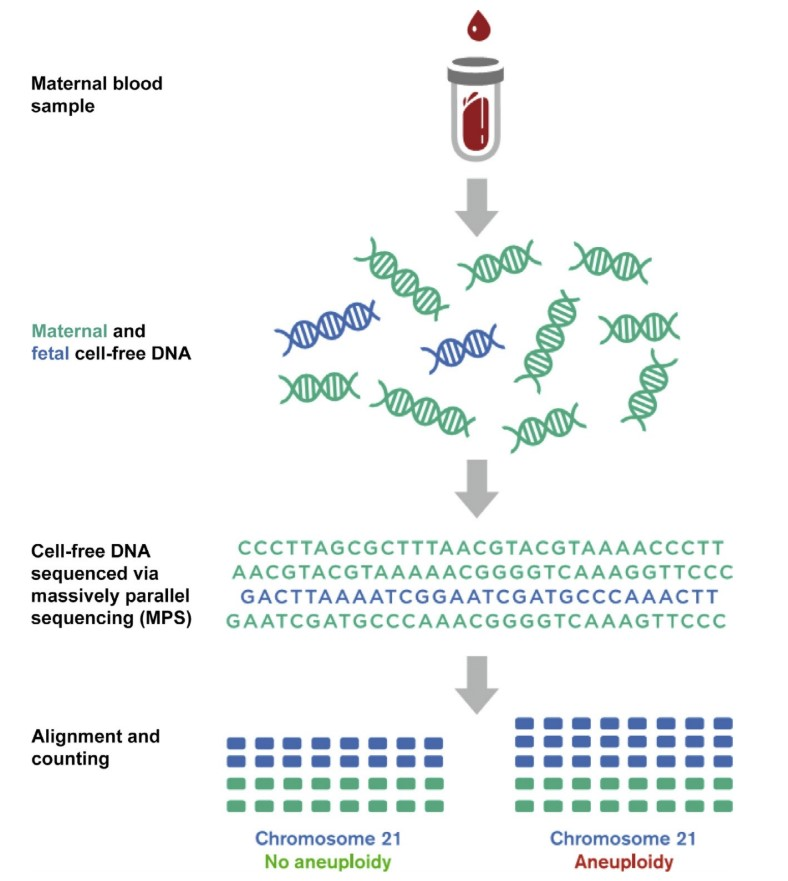
\includegraphics[width=0.5\textwidth]{clinicalAppl/NIPTkadering.jpg}
		\caption{A schematic overview of the NIPT test~\cite{NIPT}.}
		\label{fig:NIPT}
	\end{figure}
	
	Using the same method, we can also find other defects in the number of chromosomes. For example trisomy 18 (Edwards syndrome), trisomy 13 (Patau syndrome), or even in the sex chromosomes, such as XXY (Klinefelter syndrome) or lack of a second X or a Y chromosome (Turner syndrome)~\cite{NIPT}.
	
	\item \textbf{Shallow whole-genome sequencing of tumor DNA.}\newline
	It is a known fact that damaged DNA can lead to tumor development. This damage can be single bases changes but can also be a loss or gain of large DNA sequences where important genes are located. When someone is diagnosed with cancer, the knowledge of which DNA regions are lost or gained can be important to decide on treatment. 
	
	A relatively new technique to detect all gains and losses of DNA material in one single experiment is shallow whole-genome sequencing. The technique is performed as follows: DNA from the tumor is fragmented (it is broken in small pieces, eg. by a fragmentase enzyme or by high-frequency sound). These pieces are sequenced randomly, and with a mapping algorithm to the reference genome, the over- or underrepresentation of reads (as compared with a normal sample) indicates if regions of the DNA have changed, and which regions these are~\cite{SWG}.
	
	This technique is currently being optimized and validated in the laboratory of the AZ Sint-Jan hospital (in Bruges, Belgium) for analysis of DNA gains or losses important for diagnosis, follow-up and therapy of leukemia's, lymphoma's and some solid tumor types.
\end{enumerate}
%%%%%%%%%%%%%%%%%%%%%%%%%%%%%%%%%%%%%%%%%%%%%%%%%%%%%%%%%%%%%%%%%%% 
%                                                                 %
%                            CHAPTER                              %
%                                                                 %
%%%%%%%%%%%%%%%%%%%%%%%%%%%%%%%%%%%%%%%%%%%%%%%%%%%%%%%%%%%%%%%%%%% 

\chapter{Platforms for accelerating the Smith-Waterman algorithm}
\label{ch:Platforms}

As we have discussed in \ref{expl:SWanalyse} (analysis of the Smith-Waterman algorithm) the value of each cell in the matrix is only dependent on the left-upmost 3 cells. Therefore, It leads us to believe that this algorithm can be accelerated on other hardware solutions that are better equipped for parallelism than a normal CPU.

\section{Overview of possible hardware}

When designing a processing unit based on the semiconductor technology, it is always a tradeoff between efficiency and flexibility. For example, the CPU in a PC is highly flexible so that it can run any set of instructions without a lot of intervention between context changes. On the other hand, if a certain algorithm or instruction set should be executed as fast as possible, the FPGA's and ASICs are the best choices. At the extreme, an ASIC or \emph{Application Specific Integrated Circuit} can be chosen, but this means a complete chip should be designed from the ground up just for this specific application. However, an ASIC is extremely expensive to design and build, especially for small production quantities. In figure \ref{fig:effVSflex} an overview of the different options can be found.

\begin{figure}[H]
	%src=https://docs.microsoft.com/en-us/azure/machine-learning/service/media/concept-accelerate-with-fpgas/azure-machine-learning-fpga-comparison.png
	\centering
	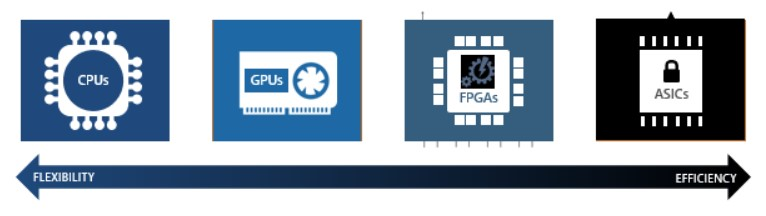
\includegraphics[width=0.75\textwidth]{elBackground/effVSflex.jpg}
	\caption{An overview of the different semiconductor technologies}
	\label{fig:effVSflex}
\end{figure}

\subsection{CPU}

The power of the CPU lies in its flexibility: it can be very easily programmed with new instructions in a short time. However, if the CPU would only run one specific algorithm for its whole lifetime, it would be terribly inefficient. Also, CPUs work sequentially, which is less suitable for algorithms that demand a large number of computations which could be done in parallel.

\begin{figure}[H]
	%src=http://www.lighterra.com/papers/modernmicroprocessors/sequential2.png
	\centering
	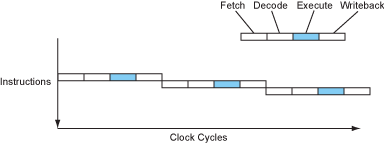
\includegraphics[width=0.75\textwidth]{elBackground/CPU.png}
	\caption{A cpu processes instructions sequentially. It could be accelerated using pipelining, but the maximum stays 1 instruction per clock cycle}
	\label{fig:cpu}
\end{figure}

Since the original implementations of the S-W algorithm on CPU, it became clear that a CPU was not the most suitable platform since it consists of a lot of operations that can be done in parallel. However, since the rise of SIMD, CPU's speed for parallel operations have improved substantially. \emph{SIMD} stands for \emph{Single Instruction Multiple Data} and makes it possible to manipulate more than 1 attribute of data with a single instruction, although be it the same instruction on all the data. CLC bio, a Danish company specialized in bioinformatics, has been able to achieve impressive speedups with a software implementation using SIMD, closing in on 200x.
%src:https://web.archive.org/web/20070811101052/http://www.clccell.com/download.html

Nowadays, MIT has published \emph{diagonalsw}, which is an implementation of S-W using the SIMD instruction set and is licensed under the open-source MIT license.

\subsection{GPU}

A GPU or \emph{Graphical Processing Unit} is a semiconductor technology which is specialized in video encoding and decoding. Since video encoding and decoding are actually glorified matrix manipulations, a GPU could also be used to manipulate all kinds of matrices. Since the Smith-Waterman algorithm is a big matrix fill in, it leads researchers to believe that it could be accelerated on a GPU. In 1997, an implementation of S-W on a GPU was published %src:  https://archive.org/details/computationalsci0000iccs_y9o8/page/230
which achieved a speedup of 2x over all previous software implementations.

At the time of writing, 11 different implementations for Smith-Waterman have been reported, 3 of which reporting a speedup over 30 times.

\subsection{FPGA}

An FPGA, or \emph{Field Programmable Gate Array}, is an integrated circuit consisting of programmable logic components. These logic components can be programmed as any logic function, such as an AND, XOR, etc. In most FPGA other elements are also found, such as memory blocks, DSP blocks, etc.

In the most basic FPGA's, the following items are present:
\begin{enumerate}
	\item CLB's, or \emph{Complex Logic Blocks}, consisting of a \emph{LookUp Table} (LUT) and a flipflop. A LUT can be programmable so that it contains any type of logic function.
	\item Programmable Interconnects have to connect the CLB's into a bigger circuit, which is also called \emph{routing}. This routing has the most influence on delays, and are also responsible for most errors.
	\item I/O blocks, which connect the internal logic inside with the outside pins of the FPGA. Most can be configured as input, output, or bidirectional.
\end{enumerate}

\begin{figure}[H]
	%src=https://evergreen.loyola.edu/dhhoe/www/FPGA_diagram.png
	\centering
	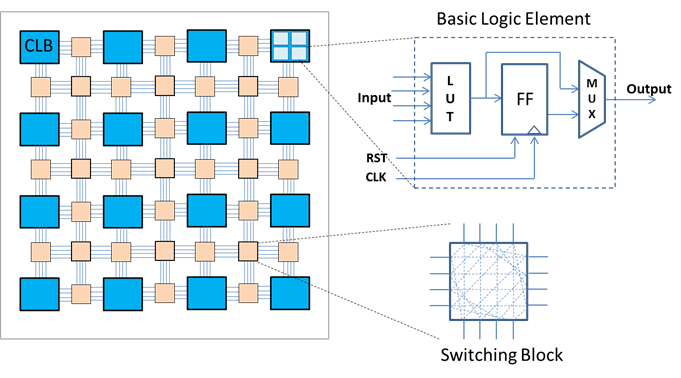
\includegraphics[width=0.75\textwidth]{elBackground/FPGA.png}
	\caption{The basic layout of an FPGA}
	\label{fig:fpga}
\end{figure}

For an implementation or design of a circuit which should be loaded in an FPGA, a \emph{Hardware Description Language} (HDL) is often the only practical choice to implement such a system, since drawing the circuits with a CAD program or by hand would take a very long time.

In a paper from 2007, an implementation of S-W with an FPGA (Virtex-4) achieved a speedup of up to 100x in comparison with a 2.2GHz Opteron processor. %src https://ft.ornl.gov/~olaf/pubs/RSSIOlafDave.pdf
A few companies have also made some implementations on FPGA in the past, e.g. Cray Inc., TimeLogics, ...
%cray: https://www.cray.com/
%timelogics: http://www.timelogic.com/

A master's thesis from 2011 by Vermij E. (university, city, country) has a detailed analysis of an FPGA based Smith-Waterman implementation. In other papers, it was found that the performance per Watt level for an FPGA implementation is better than a GPU or CPU by a factor of 12-21 times.

\section{Hardware selection}

As the hardware the ZCU 104 evaluation kit was selected, which has an MPSoC onboard. An MPSoC (or \emph{Multi-Processor System on Chip}) is an integrated circuit that contains multiple microprocessors. This means that both a processor and programmable hardware is available.

\begin{figure}[H]
	%src=https://evergreen.loyola.edu/dhhoe/www/FPGA_diagram.png
	\centering
	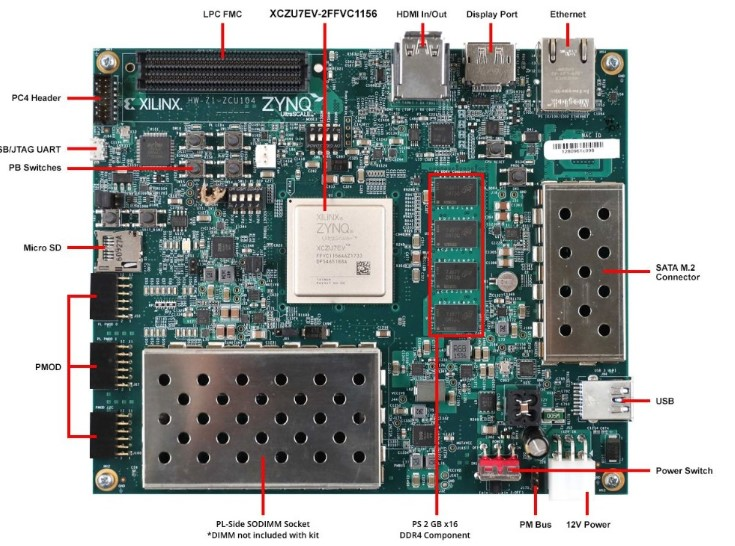
\includegraphics[width=0.75\textwidth]{elBackground/hardware.jpg}
	\caption{An overview of the hardware available on the ZCU 104 MPSoC evaluation kit}
	\label{fig:hardware}
\end{figure}

Reasons for choosing the ZCU 104 evaluation kit:
\begin{enumerate}
	\item An MPSoC is present, which will be used the host to application;
	\item Both a USB and Ethernet interface is available, which makes it easy to communicate with the target board;
	\item An operating system can be run on the board (a Red Hat Linux distribution). This means we won't have to worry about implementing FAT or Ethernet stacks;
	\item 16 times 2 gigabytes of RAM is available, which can come in handy when implementing big structures, like the alignment matrix;
	\item It was available at the Brno University of Technology.
\end{enumerate}

\subsection{Recent advances in High-Level Synthesis}

When programming an FPGA, an HDL is often used. However, if a specific implementation already exists in a programming language, it often has to be reimplemented from scratch in HDL to load it on the FPGA. Therefore people have been trying to make a compiler that compiles normal C code into HDL. This "compiler" is called HLS, or \emph{ High-Level Synthesis}. In recent years, HLS became popular as an alternative for designing and implementing a complex system that should be run on an FPGA.

When researching in the known literature, no implementation using HLS for the Smith-Waterman algorithm was found. This leads us to believe that this is still an unexplored area.

\subsection{Platform communication}

Initially, it seemed important that there is good communication between the board and the host to load and unload sequences since we didn't want the communication to become the bottleneck. However, when using S-W for genome mapping, this won't be an issue since the time it takes to map a read takes a lot longer than to transfer it.

In the end, no direct communication with the board was implemented. It seemed sufficient to just load the reads with the genome on an SD card, and insert this in the board. After the mapping process, the mapped reads are available on the same SD card. However, if this program would be used in practice, it doesn't seem practical to constantly change out the SD card. Therefore, another solution should be found. A possible solution could be by using the Ethernet stack available as part of the OS, so we could easily use FTP for on and offloading from and to the board.


%%%%%%%%%%%%%%%%%%%%%%%%%%%%%%%%%%%%%%%%%%%%%%%%%%%%%%%%%%%%%%%%%%% 
%                                                                 %
%                            CHAPTER                              %
%                                                                 %
%%%%%%%%%%%%%%%%%%%%%%%%%%%%%%%%%%%%%%%%%%%%%%%%%%%%%%%%%%%%%%%%%%% 

\chapter{HLS and SDSoC learning tools}
\label{ch:InitDiff}

\textit{Disclaimer: The purpose of this chapter is to show the learning tools I used to achieve a suitable implementation for the genome mapping problem. New programming techniques such as HLS, SDSoC \dots were familiarized. This chapter might be less applicable if the reader is interested in the science and implementation approach of the genome mapping problem, but can be of interest if the reader is also new to the mentioned programming techniques.}

\section{Using Vivado HLS and Xilinx SDK}

\subsection{Learning HLS in examples}
\label{HLS}

To learn HLS, I used learning materials from Mr. Martinek, who teaches HLS at the Brno University of Technology. It contains a theory part,  and also hands-on lab examples. These labs were worth exploring in this thesis since they contain most concepts of HLS.

\paragraph{Lab1: BASIC WORKFLOW} 
\begin{itemize}
	\item How to start a new project;
	\item What the difference is between a source and a test bench;
	\item The properties of the available IDE when designing in HLS;
	\item How to simulate the sources using the test benches;
	\item Generate Gantt charts and how to analyze them;
	\item Where to fiend the resulting VHDL code;
	\item What the co-simulation is and why it is used;
	\item Where to view the resulting simulation waveforms;
	\item How to export your design as an IP;
	\item It is possible to compare multiple solutions for a problem;
	\item How to set a directive (such as unrolling a loop).
\end{itemize}

\paragraph{lab2: EXPLORING DATA TYPES using an FIR filter}
\begin{itemize}
	\item When to use the floating point or fixed point representation;
	\item How to enable saturation when using fixed point;
	\item How to do calculations that normally would result in an overflow using a fixed point. This can be done by lowering the resolution (dropping LSBs) so the result can still be stored in the same bit width.
\end{itemize}

\paragraph{lab3: INTERFACES} 
\begin{itemize}
	\item The basic argument-level interfaces and their differences, such as ap\_vld, ap\_none, and ap\_hs;
	\item A block-level interface of a pipelined component (pipeline in the top function).
\end{itemize}


\paragraph{lab4: ARRAYS}
\begin{itemize}
	\item Sequential running of a design;
	\item How to pipeline an internal loop;
	\item What a rewind parameter is;
	\item How to do top-function pipelining;
	\item The array-map technique;
	\item How to partition arrays (cyclic and complete);
	\item How to reshape arrays
\end{itemize}

\subsection{Learning how to program target board}

At first, the Xilinx SDK was used to program the board. However, it was found to be unpractical to use, because after programming a "Hello World" application it became clear that it would be bare-metal. This would mean there would be a need to implement a FAT or Ethernet stack ourselves.
Therefore the SDSoC IDE was used for programming the target board, which structures the application on top of an operating system. This operating system takes care of the Ethernet and FAT stacks.

\section{SDSoC}

SDSoC is an IDE developed by Xilinx which is specialized in programming MPSoCs. It is based on the Eclipse IDE, so most of its features are familiar to most programmers. 

The power of SDSoC lays in the ability to transfer functions from software to programmable logic easily. It can be done with just the click of a button. Then, the functions marked for hardware (written in C) will be fitted in the programmable logic using the HLS compiler. However, the syntax is not always accepted since HLS cannot implement every possible programming technique in C yet.

As mentioned earlier, in this implementation we will work on a Linux distribution.

\subsection{Learning process on matrix multiplication example in SDSoC}

To learn MPSoC and the SDSoC IDE, Xilinx' online available materials were used available at their GitHub page, which includes some hands-on assignments. The assignments use a matrix multiplication example, preinstalled with SDSoC.
%TODO: link github page

\paragraph{lab1: INTRODUCTION}
\begin{itemize}
	\item Basic workflow: how to create a project, select platform, configure bare-metal or using an operating system, loading the examples;
	\item Working with hardware accelerators: mark a function for hardware, data motion network report;
	\item How to run the project
\end{itemize}

\paragraph{lab2: PERFORMANCE ESTIMATION} 
\begin{itemize}
	\item Analyse the software solutions;
	\item How to view rescource utilization after comilation; 
	\item Comparing software and hardware implementations
\end{itemize}

\paragraph{lab3: DMA}
\begin{itemize}
	\item There are directives to configure the way data is transferred between the software processor and the programmable logic:
	\begin{enumerate}
		\item ACP: Hardware functions have cache-coherent access to DDR via the PS L2 cache.
		\item AFI (HP):    Hardware functions have fast non-cache coherent access to DDR via the PS memory controller.
		\item GP: The processor directly writes/reads data to/from hardware function. This would be inefficient for large data transfers.
	\end{enumerate}
	This lab also covers how to set these directives.
	
	\item How to find more info on errors by using the log files
	
	\item the difference between the malloc() and sds\_alloc() functions. The hardware functions can only access the physical address space and not the virtual one used by the software. Therefore, the sds\_alloc() function was created to skip this virtual memory translation in software.
\end{itemize}

\paragraph{lab4: DIRECTIVES} This lab covers how to set directives to speed up the hardware functions. Which directives to set and what they do, was already covered in the HLS labs at \ref{HLS}.

\paragraph{lab5: TASK-LEVEL PIPELINING} By using task-level pipelining I was able to achieve a speedup of 3 times with a 32x32 matrix multiplication.

\paragraph{lab6: DEBUG} In this lab the onboard debugging is covered.

\paragraph{lab7: HARDWARE DEBUG} 
Using the trace feature in the SDSoC, it is possible to analyze what the application is doing? (software, hardware, transfer, or receive).

%%%%%%%%%%%%%%%%%%%%%%%%%%%%%%%%%%%%%%%%%%%%%%%%%%%%%%%%%%%%%%%%%%% 
%                                                                 %
%                            CHAPTER                              %
%                                                                 %
%%%%%%%%%%%%%%%%%%%%%%%%%%%%%%%%%%%%%%%%%%%%%%%%%%%%%%%%%%%%%%%%%%% 

\chapter{Initial approach with pure Smith-Waterman}

\section{The concept}

\section{System implementation}

\section{Possible initial speedups}

\section{Problems with this initial approach}

computational complexity: O(mn)


%%%%%%%%%%%%%%%%%%%%%%%%%%%%%%%%%%%%%%%%%%%%%%%%%%%%%%%%%%%%%%%%%%% 
%                                                                 %
%                            CHAPTER                              %
%                                                                 %
%%%%%%%%%%%%%%%%%%%%%%%%%%%%%%%%%%%%%%%%%%%%%%%%%%%%%%%%%%%%%%%%%%% 

\chapter{Acccelerating the software implementation using HLS}

\section{Analysing software performance}

In the SDSoC environment, it is possible to analyse the software running on the SoC chip using a TCF profiler. After running this analysis, the TCF profiler returns an overview of the functions, sorted on the amount of time spent when running. The analysis is shown in figure \ref{fig:softwareFunctionUsage}

\begin{figure}[H]
	\centering
	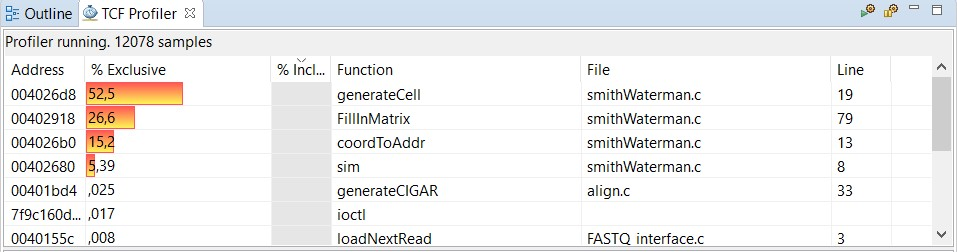
\includegraphics[width=0.75\textwidth]{speedup/softwareFunctionUsage.jpg}
	\caption{a TCF profile of the software implementation}
	\label{fig:softwareFunctionUsage}
\end{figure}

When examining this analysis, we should keep in mind that the generateCell, coordToAddr and sim functions are inline functions used in the FillInMatrix method. Just as suspected the software spends almost all of its time in these methods, so it's worth it to try to accelerate these functions.

\section{Recoding parts of the software to be more hardware friendly}

Back in 2011, Vermij E. did a thesis on RVE (recursive variable expansion). In it, he discusses the most efficient ways to program a processing element to generate one value in the alignment matrix. His results can be found in figure \ref{fig:PE}. 

\begin{figure}[H]
	%src=file:///D:/Erasmus/thesis/interessante%20papers/masterthesis%20Smith-Waterman%20op%20FPGA%20(TU%20Delft).pdf
	\centering
	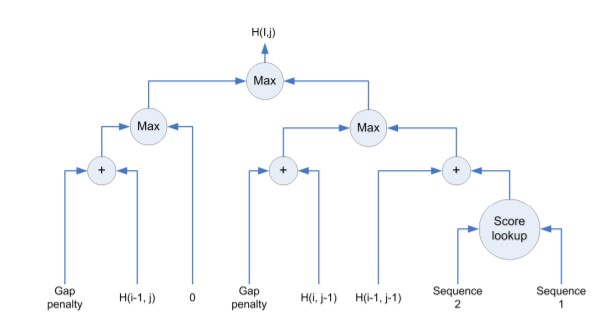
\includegraphics[width=0.75\textwidth]{speedup/PE.jpg}
	\caption{The optimal processing found in the thesis from Vermij E.}
	\label{fig:PE}
\end{figure}

It seemed like a good idea to reimplement the generatecell function, using this newly found scheme. However, it is also important to keep track of where the value comes from. Therefore, the following (new) code was adopted for generating a cell:

\begin{lcverbatim}
//calculate the possible  values
CELL diagonalCELL = { diagonal.value + sim(refVal, seqVal), 1 };
CELL leftCELL = { left.value - gp, 2 };
CELL upCELL = { up.value - gp, 3 };
CELL zeroCELL = { 0, 0 };

CELL upstreamA = (leftCELL.value > upCELL.value) ? leftCELL : upCELL;
CELL upstreamB = (diagonalCELL.value > zeroCELL.value) ? 
					diagonalCELL : zeroCELL;

CELL newCell = (upstreamA.value > upstreamB.value) ? upstreamA : upstreamB;

//Return the cell:
return newCell;
\end{lcverbatim}

Where the second attribute in the CELL type is the direction.

\section{Hardware acceleration}

It turns out, HLS does not support in/out matrix to memory yet.

slices

direction of matrix (first column then row).

Bitwidth of (packed) data on axi master must be power of 2. => change the int to int16\_t and direction to uint16\_t (really wastefull towards memory) but no other choice without major remodel.

\section{Comparison with the software}
%%%%%%%%%%%%%%%%%%%%%%%%%%%%%%%%%%%%%%%%%%%%%%%%%%%%%%%%%%%%%%%%%%%% 
%                                                                 %
%                            CHAPTER                              %
%                                                                 %
%%%%%%%%%%%%%%%%%%%%%%%%%%%%%%%%%%%%%%%%%%%%%%%%%%%%%%%%%%%%%%%%%%% 

\chapter{implementation results and speedup}

...
%%%%%%%%%%%%%%%%%%%%%%%%%%%%%%%%%%%%%%%%%%%%%%%%%%%%%%%%%%%%%%%%%%% 
%                                                                 %
%                            CHAPTER                              %
%                                                                 %
%%%%%%%%%%%%%%%%%%%%%%%%%%%%%%%%%%%%%%%%%%%%%%%%%%%%%%%%%%%%%%%%%%% 

\chapter{Conclusion and future research}

Gap opening and extension

BFAST algorithm

BASE type memory efficient

FTP for easy on and offloading the data

SEQ\_INDEX type maken memory efficient (75-300)


% Bibliografie: referenties. De items zitten in bibliografie.bib
%%%%%%%%%%%%%%%%%%%%%%%%%%%%%%%%%%%%%%%%%%%%%%%%%%%%%%%%%%%%%%%%%
% Indien je ook de niet geciteerde werken in je bibliografie wil opnemen, commentarieer dan onderstaande regel uit!
%\nocite{*}
\bibliographystyle{apalike}
\bibliography{bibliografie}

% Eventueel enkele appendices
%%%%%%%%%%%%%%%%%%%%%%%%%%%%%%
\appendix
\chapter{Implementation code}

The implementation code can also be found on Github: \href{https://github.com/robinno/refGenMapping}{https://github.com/robinno/refGenMapping}

\section{Filesystem organization}

To keep the code manageable, it was split up in multiple files. These files were organized in the directory structure as seen in figure \ref{fig:dirStruct}

\begin{figure}[H]
	\centering
	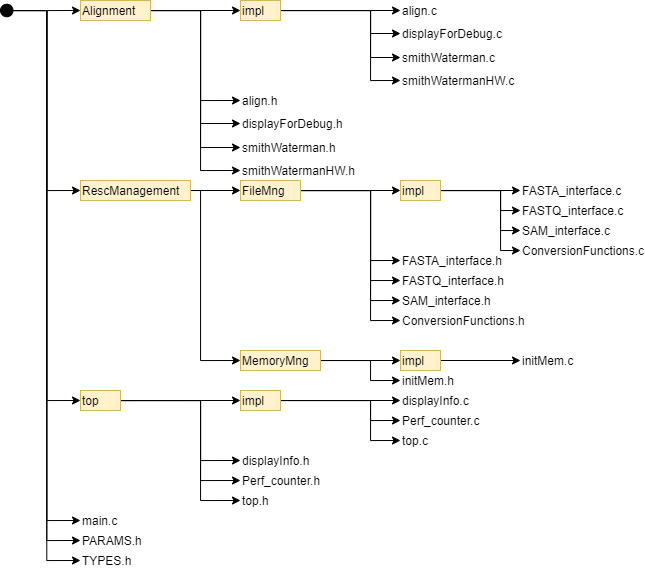
\includegraphics[width=0.8\textwidth]{code/dirStructure.png}
	\caption{The used directory structure in the implementation. Directories are colored in yellow.}
	\label{fig:dirStruct}
\end{figure}

\section{Code}
%listing all code files

{\setstretch{1.0} %interlinie afstand
	
\textbf{PARAMS.h}
\lstinputlisting[language=C]{sourceCode/PARAMS.h}
\textbf{TYPES.h}
\lstinputlisting[language=C]{sourceCode/TYPES.h}
\textbf{main.c}
\lstinputlisting[language=C]{sourceCode/main.c}


\textbf{top.h}
\lstinputlisting[language=C]{sourceCode/top/top.h}
\textbf{top.c}
\lstinputlisting[language=C]{sourceCode/top/impl/top.c}
\textbf{displayInfo.h}
\lstinputlisting[language=C]{sourceCode/top/displayInfo.h}
\textbf{displayInfo.c}
\lstinputlisting[language=C]{sourceCode/top/impl/displayInfo.c}
\textbf{Perf\_counter.h}
\lstinputlisting[language=C]{sourceCode/top/Perf_counter.h}
\textbf{Perf\_counter.c}
\lstinputlisting[language=C]{sourceCode/top/impl/Perf_counter.c}


\textbf{ConversionFunctions.h}
\lstinputlisting[language=C]{sourceCode/RescManagement/FileMng/ConversionFunctions.h}
\textbf{ConversionFunctions.c}
\lstinputlisting[language=C]{sourceCode/RescManagement/FileMng/impl/ConversionFunctions.c}
\textbf{FASTA\_interface.h}
\lstinputlisting[language=C]{sourceCode/RescManagement/FileMng/FASTA_interface.h}
\textbf{FASTA\_interface.c}
\lstinputlisting[language=C]{sourceCode/RescManagement/FileMng/impl/FASTA_interface.c}
\textbf{FASTQ\_interface.h}
\lstinputlisting[language=C]{sourceCode/RescManagement/FileMng/FASTQ_interface.h}
\textbf{FASTQ\_interface.c}
\lstinputlisting[language=C]{sourceCode/RescManagement/FileMng/impl/FASTQ_interface.c}
\textbf{SAM\_interface.h}
\lstinputlisting[language=C]{sourceCode/RescManagement/FileMng/SAM_interface.h}
\textbf{SAM\_interface.c}
\lstinputlisting[language=C]{sourceCode/RescManagement/FileMng/impl/SAM_interface.c}


\textbf{initMem.h}
\lstinputlisting[language=C]{sourceCode/RescManagement/MemoryMng/initMem.h}
\textbf{initMem.c}
\lstinputlisting[language=C]{sourceCode/RescManagement/MemoryMng/impl/initMem.c}


\textbf{align.h}
\lstinputlisting[language=C]{sourceCode/Alignment/align.h}
\textbf{align.c}
\lstinputlisting[language=C]{sourceCode/Alignment/impl/align.c}
\textbf{displayForDebug.h}
\lstinputlisting[language=C]{sourceCode/Alignment/displayForDebug.h}
\textbf{displayForDebug.c}
\lstinputlisting[language=C]{sourceCode/Alignment/impl/displayForDebug.c}
\textbf{smithWaterman.h}
\lstinputlisting[language=C]{sourceCode/Alignment/smithWaterman.h}
\textbf{smithWaterman.c}
\lstinputlisting[language=C]{sourceCode/Alignment/impl/smithWaterman.c}
\textbf{smithWatermanHW.h}
\lstinputlisting[language=C]{sourceCode/Alignment/smithWatermanHW.h}
\textbf{smithWatermanHW.c}
\lstinputlisting[language=C]{sourceCode/Alignment/impl/smithWatermanHW.c}
} %end line stretch




% Back cover: change according to the correct campus
% 
\includepdf{private/back_fiiw_denayer.pdf}
% 
\includepdf{private/back_fiiw_denayer_eng.pdf} % For the english version
%
\includepdf{private/back_fiiw_geel.pdf}
% 
\includepdf{private/back_fiiw_geel_eng.pdf} % For the english version
%
\includepdf{private/back_fiiw_gent.pdf}
% 
\includepdf{private/back_fiiw_ghent_eng.pdf} % For the english version

\includepdf{private/back_fiiw_brugge.pdf}
% 
\includepdf{private/back_fiiw_bruges_eng.pdf} % For the english version
%
\includepdf{private/back_fiiw_groept.pdf}
% \includepdf{private/back_fiiw_groupt_eng.pdf} % For the english version

\end{document}
